\newpage
\section*{Domain Discovery}\label{sec:SuppDomainDiscovery}

Using the directionality indices computed on at 10kb resolution map, we computed domains by selecting the regions with the top
$10\%$ directionality bias.  Domains were further refined by intersecting between replicates and discarding non-overlapping
domains, leaving a small, conserved subset.  Overlaps between window sizes and replicates are shown in the figures below.

\subsection*{Domain Conservation}\label{sec:domainConservation}

\begin{figure}[H]
  \caption{Conserved Domains between IMR90 Replicates}
  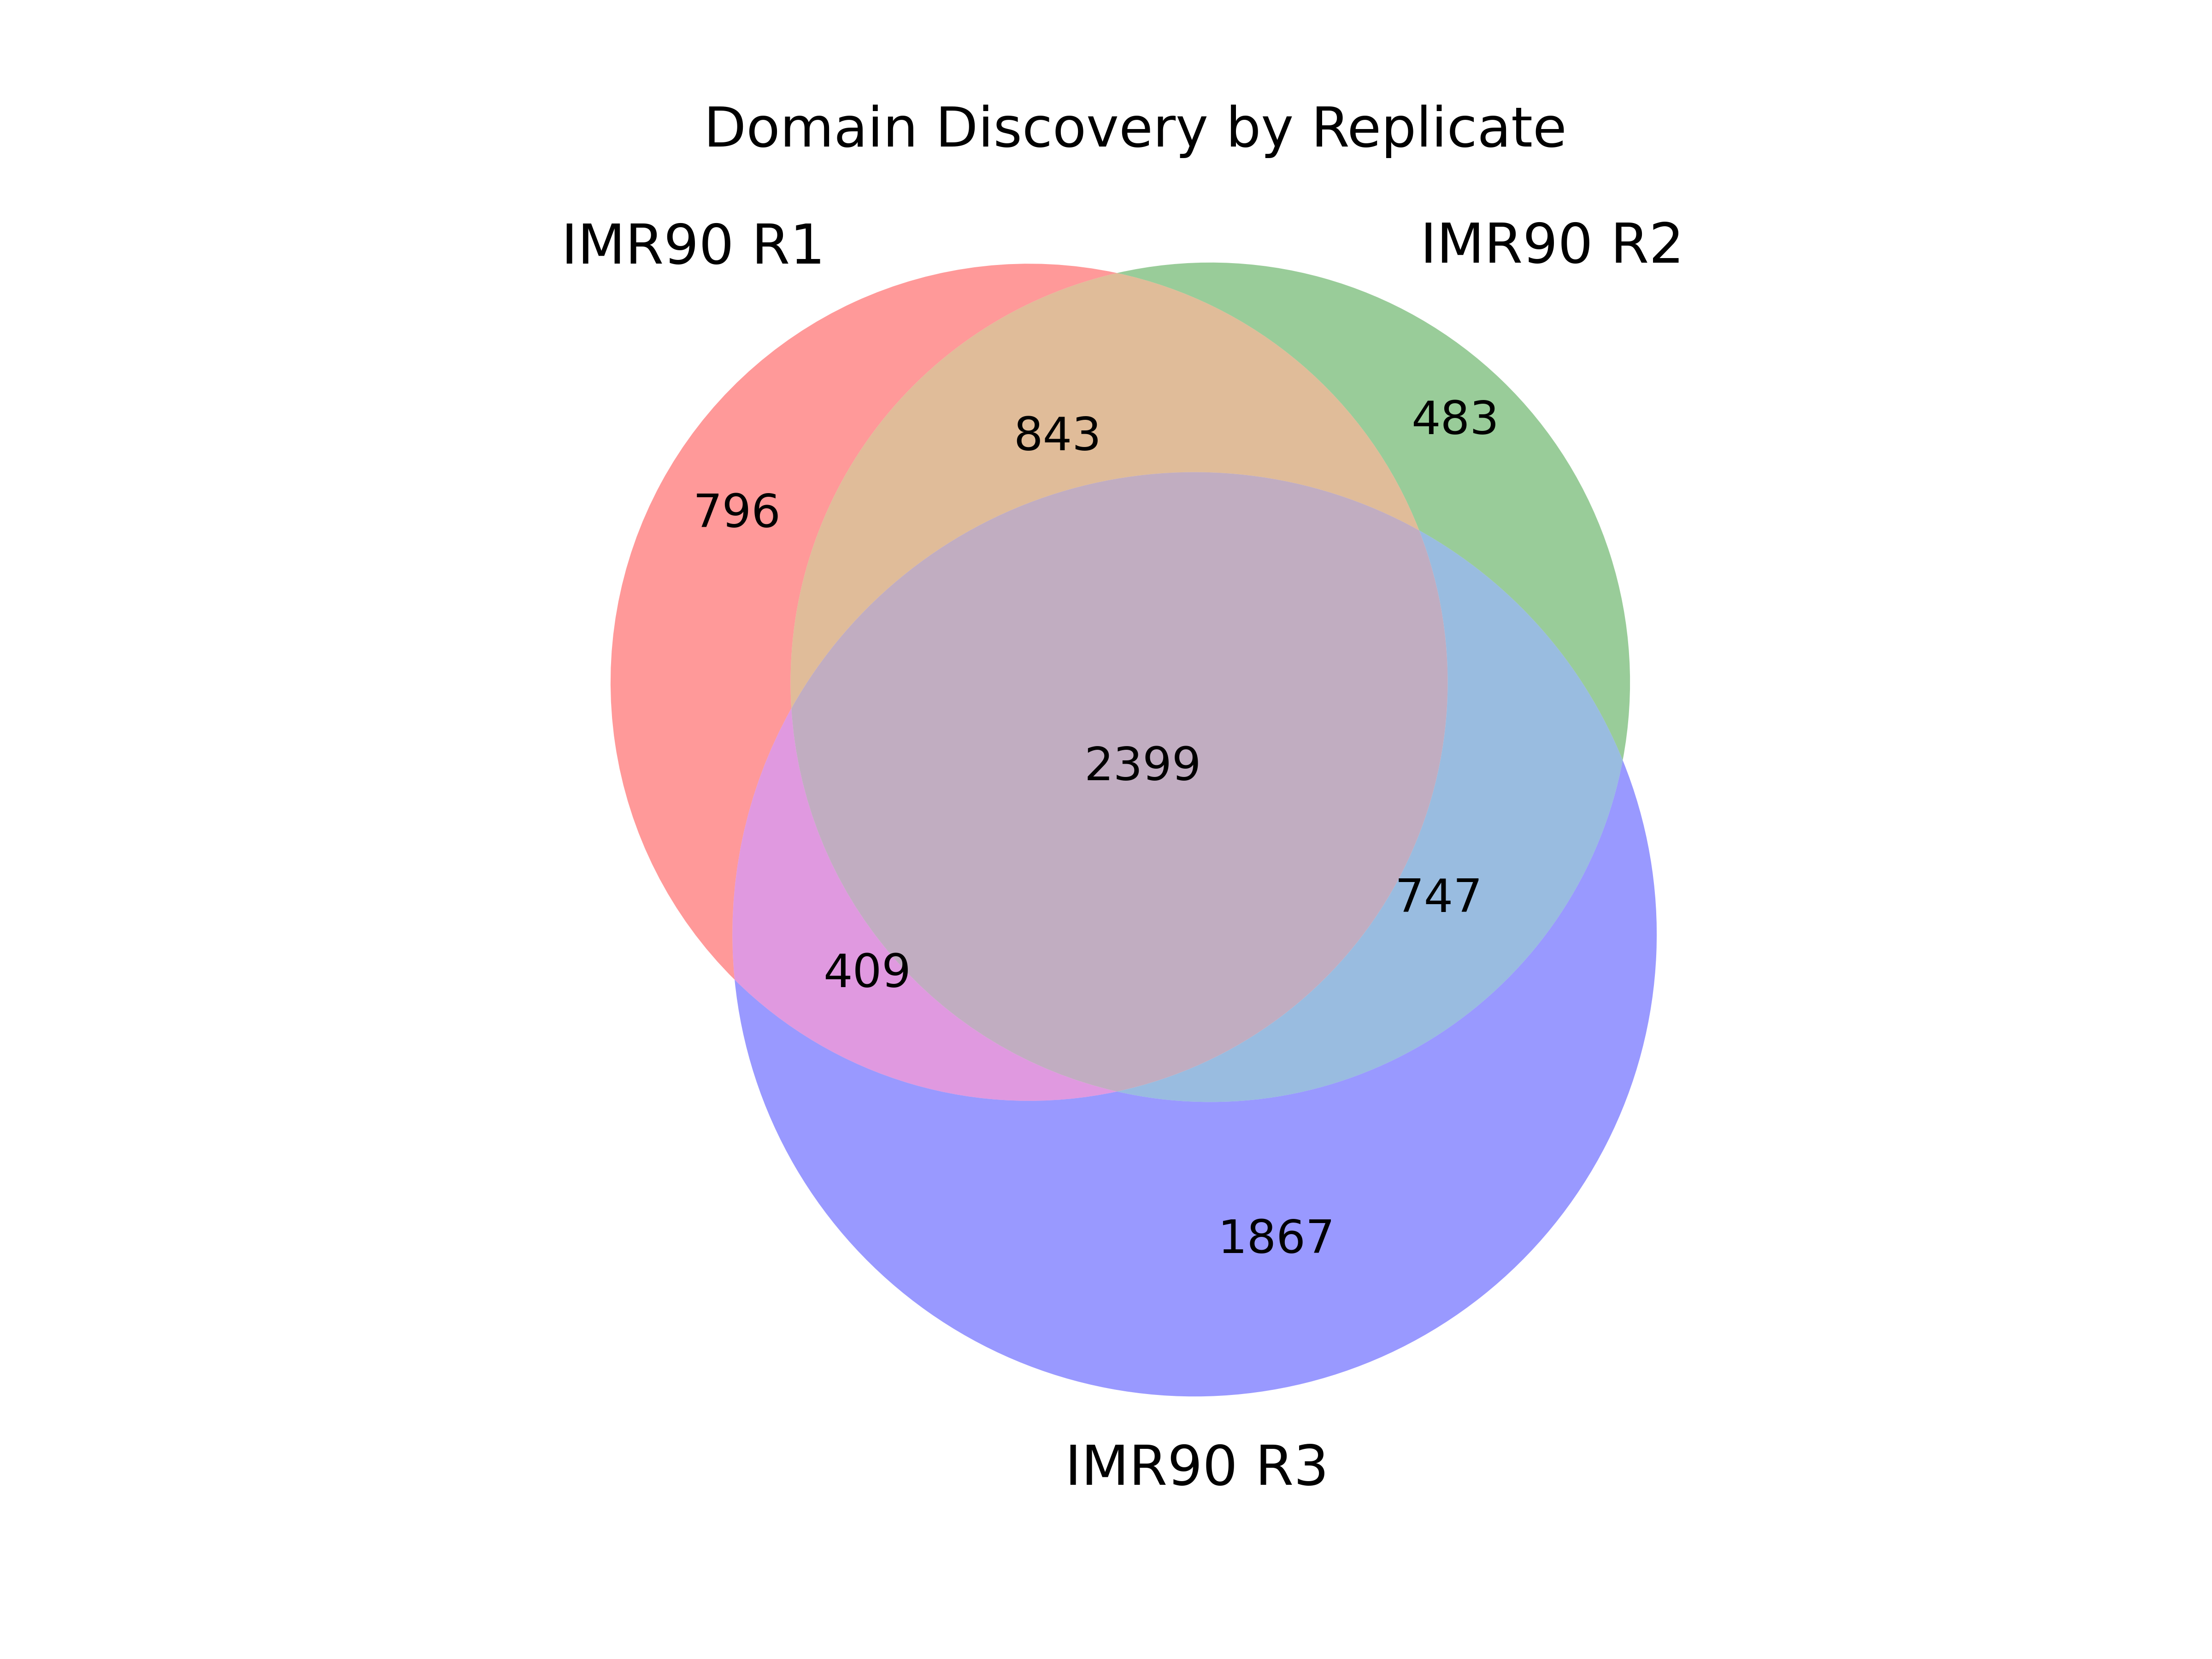
\includegraphics[width=\textwidth]{figures/supplementary/domains/venn3.png}\label{fig:SuppVenn3}
  \medskip
  \small
  Domain conservation between the first three IMR90 replicates.  The window size here is 200kb for each
  replicate.
\end{figure}

\begin{figure}[H]
  \caption{Domain Size Histograms}
  \begin{minipage}{0.5\textwidth}%
    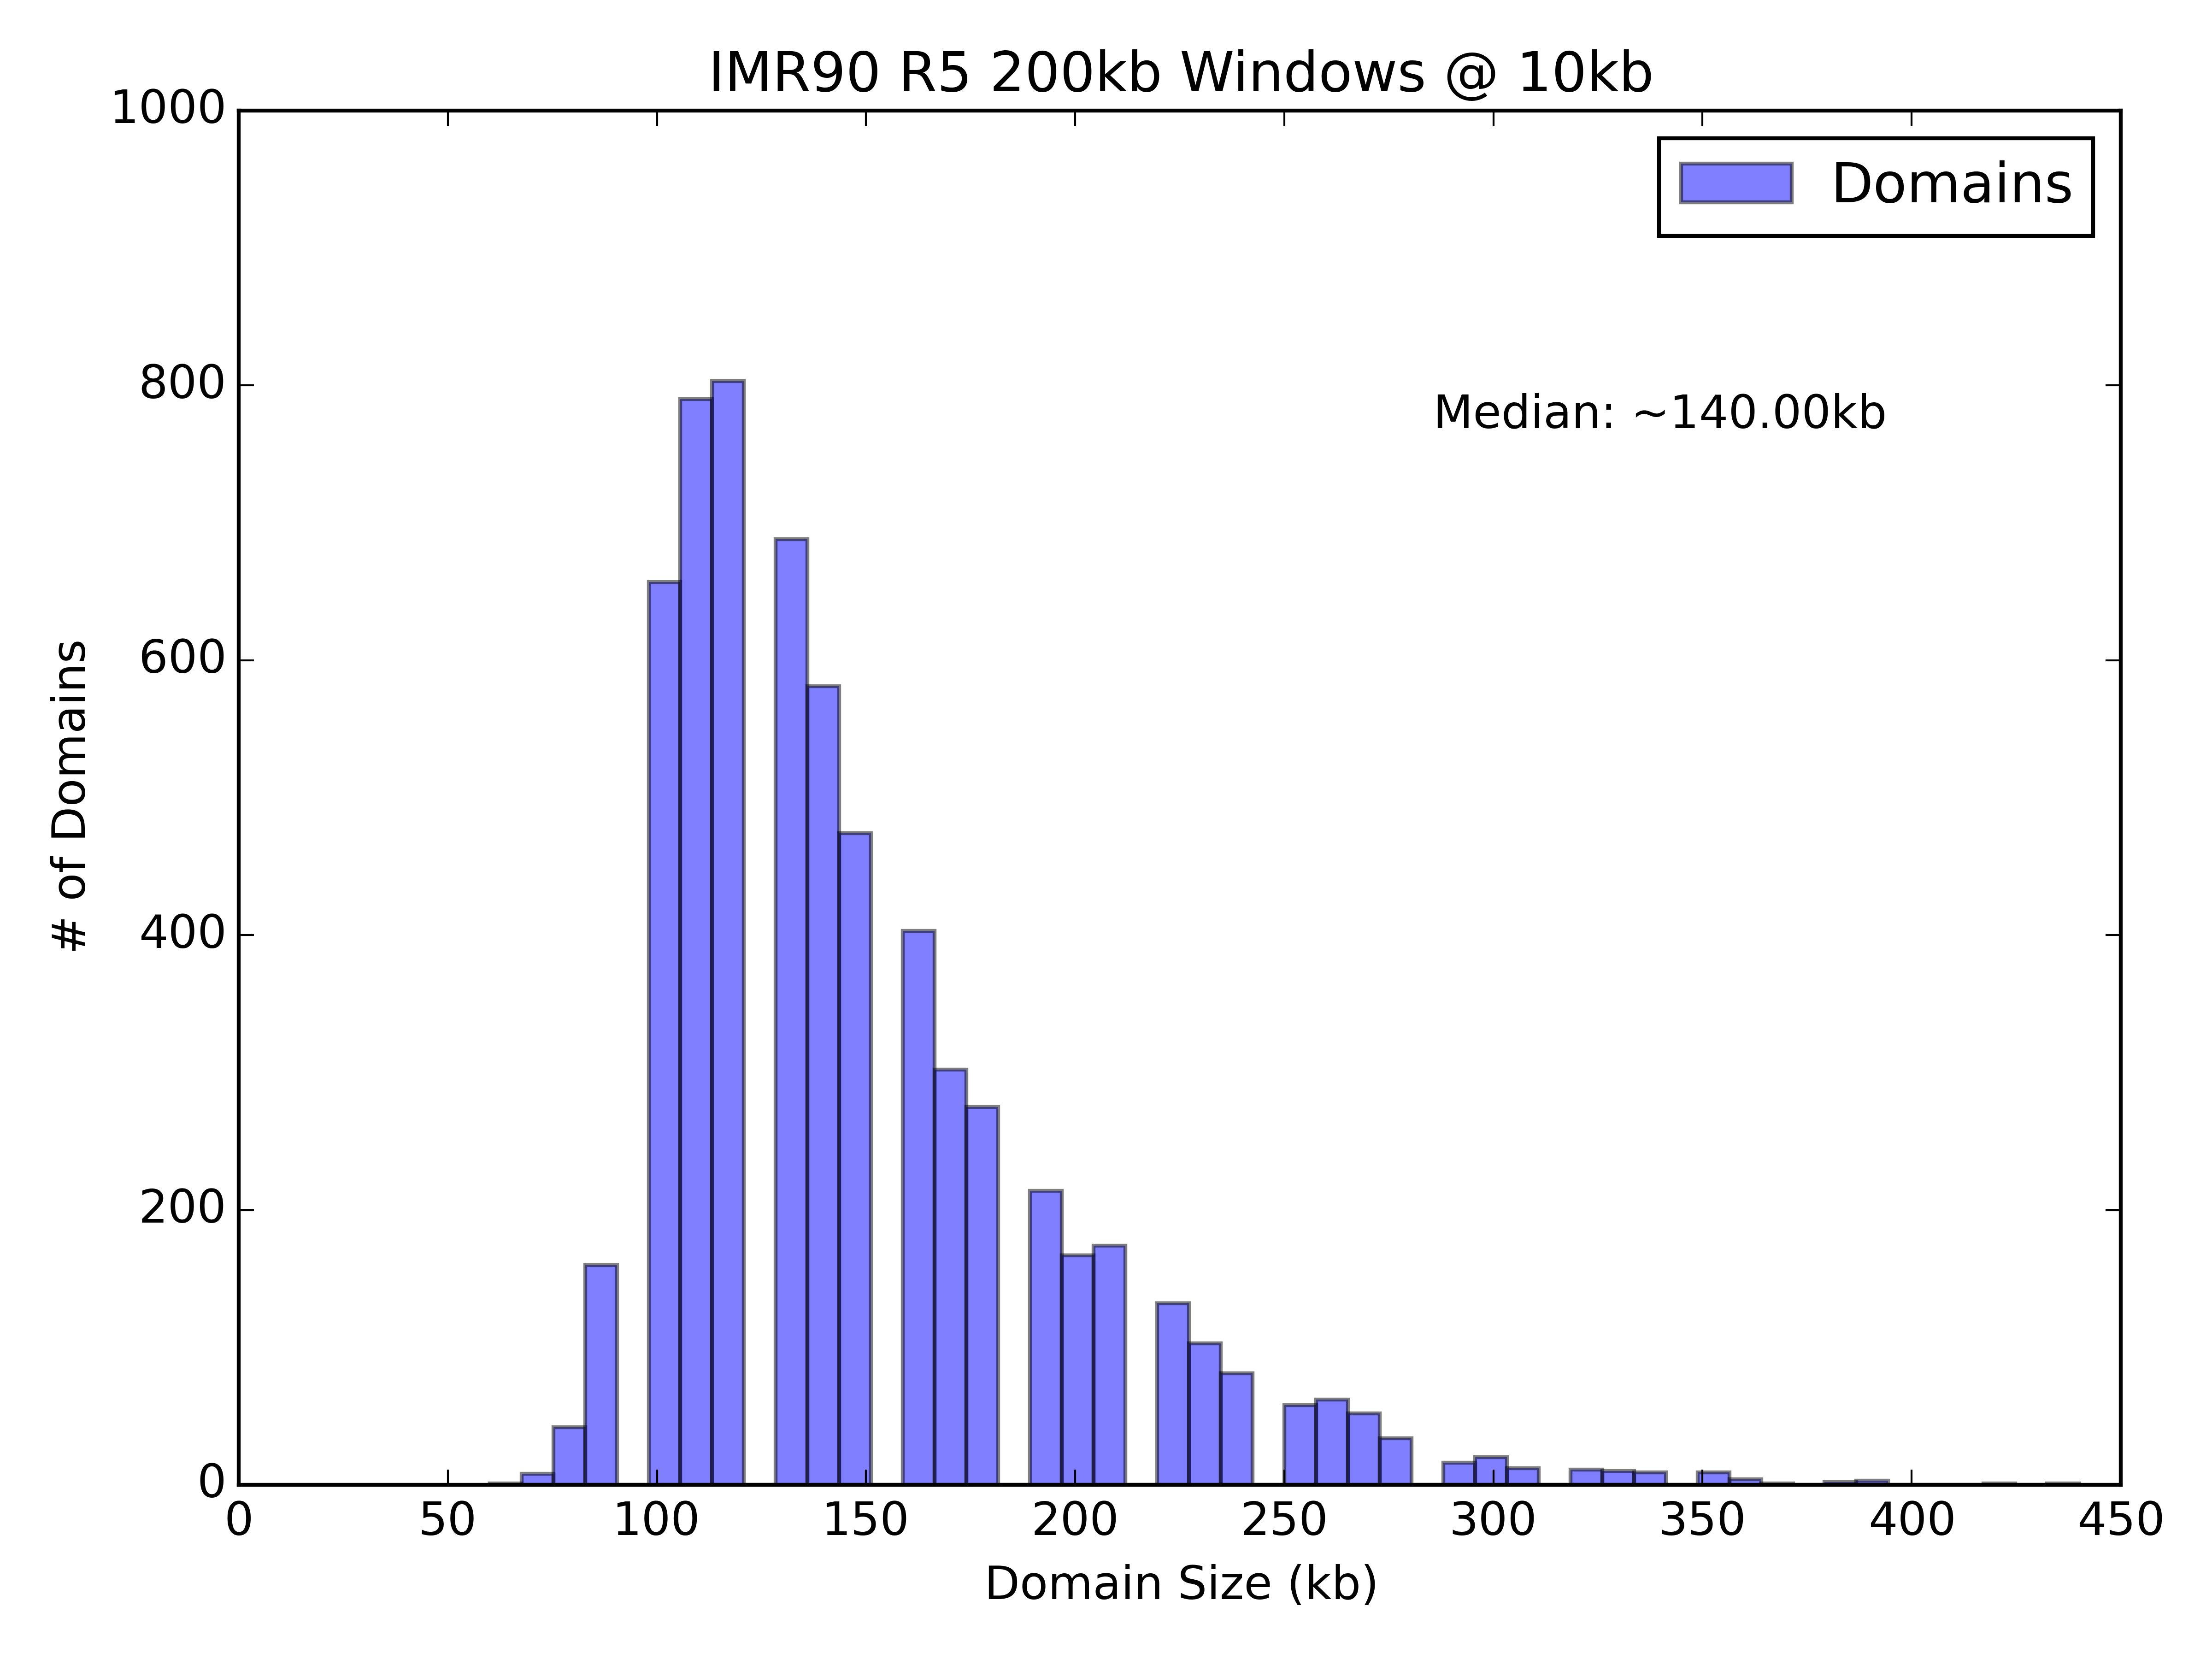
\includegraphics[width=\textwidth]{./figures/supplementary/domains/size200kb.png}
  \end{minipage}%
  \hfill
  \begin{minipage}{0.5\textwidth}
    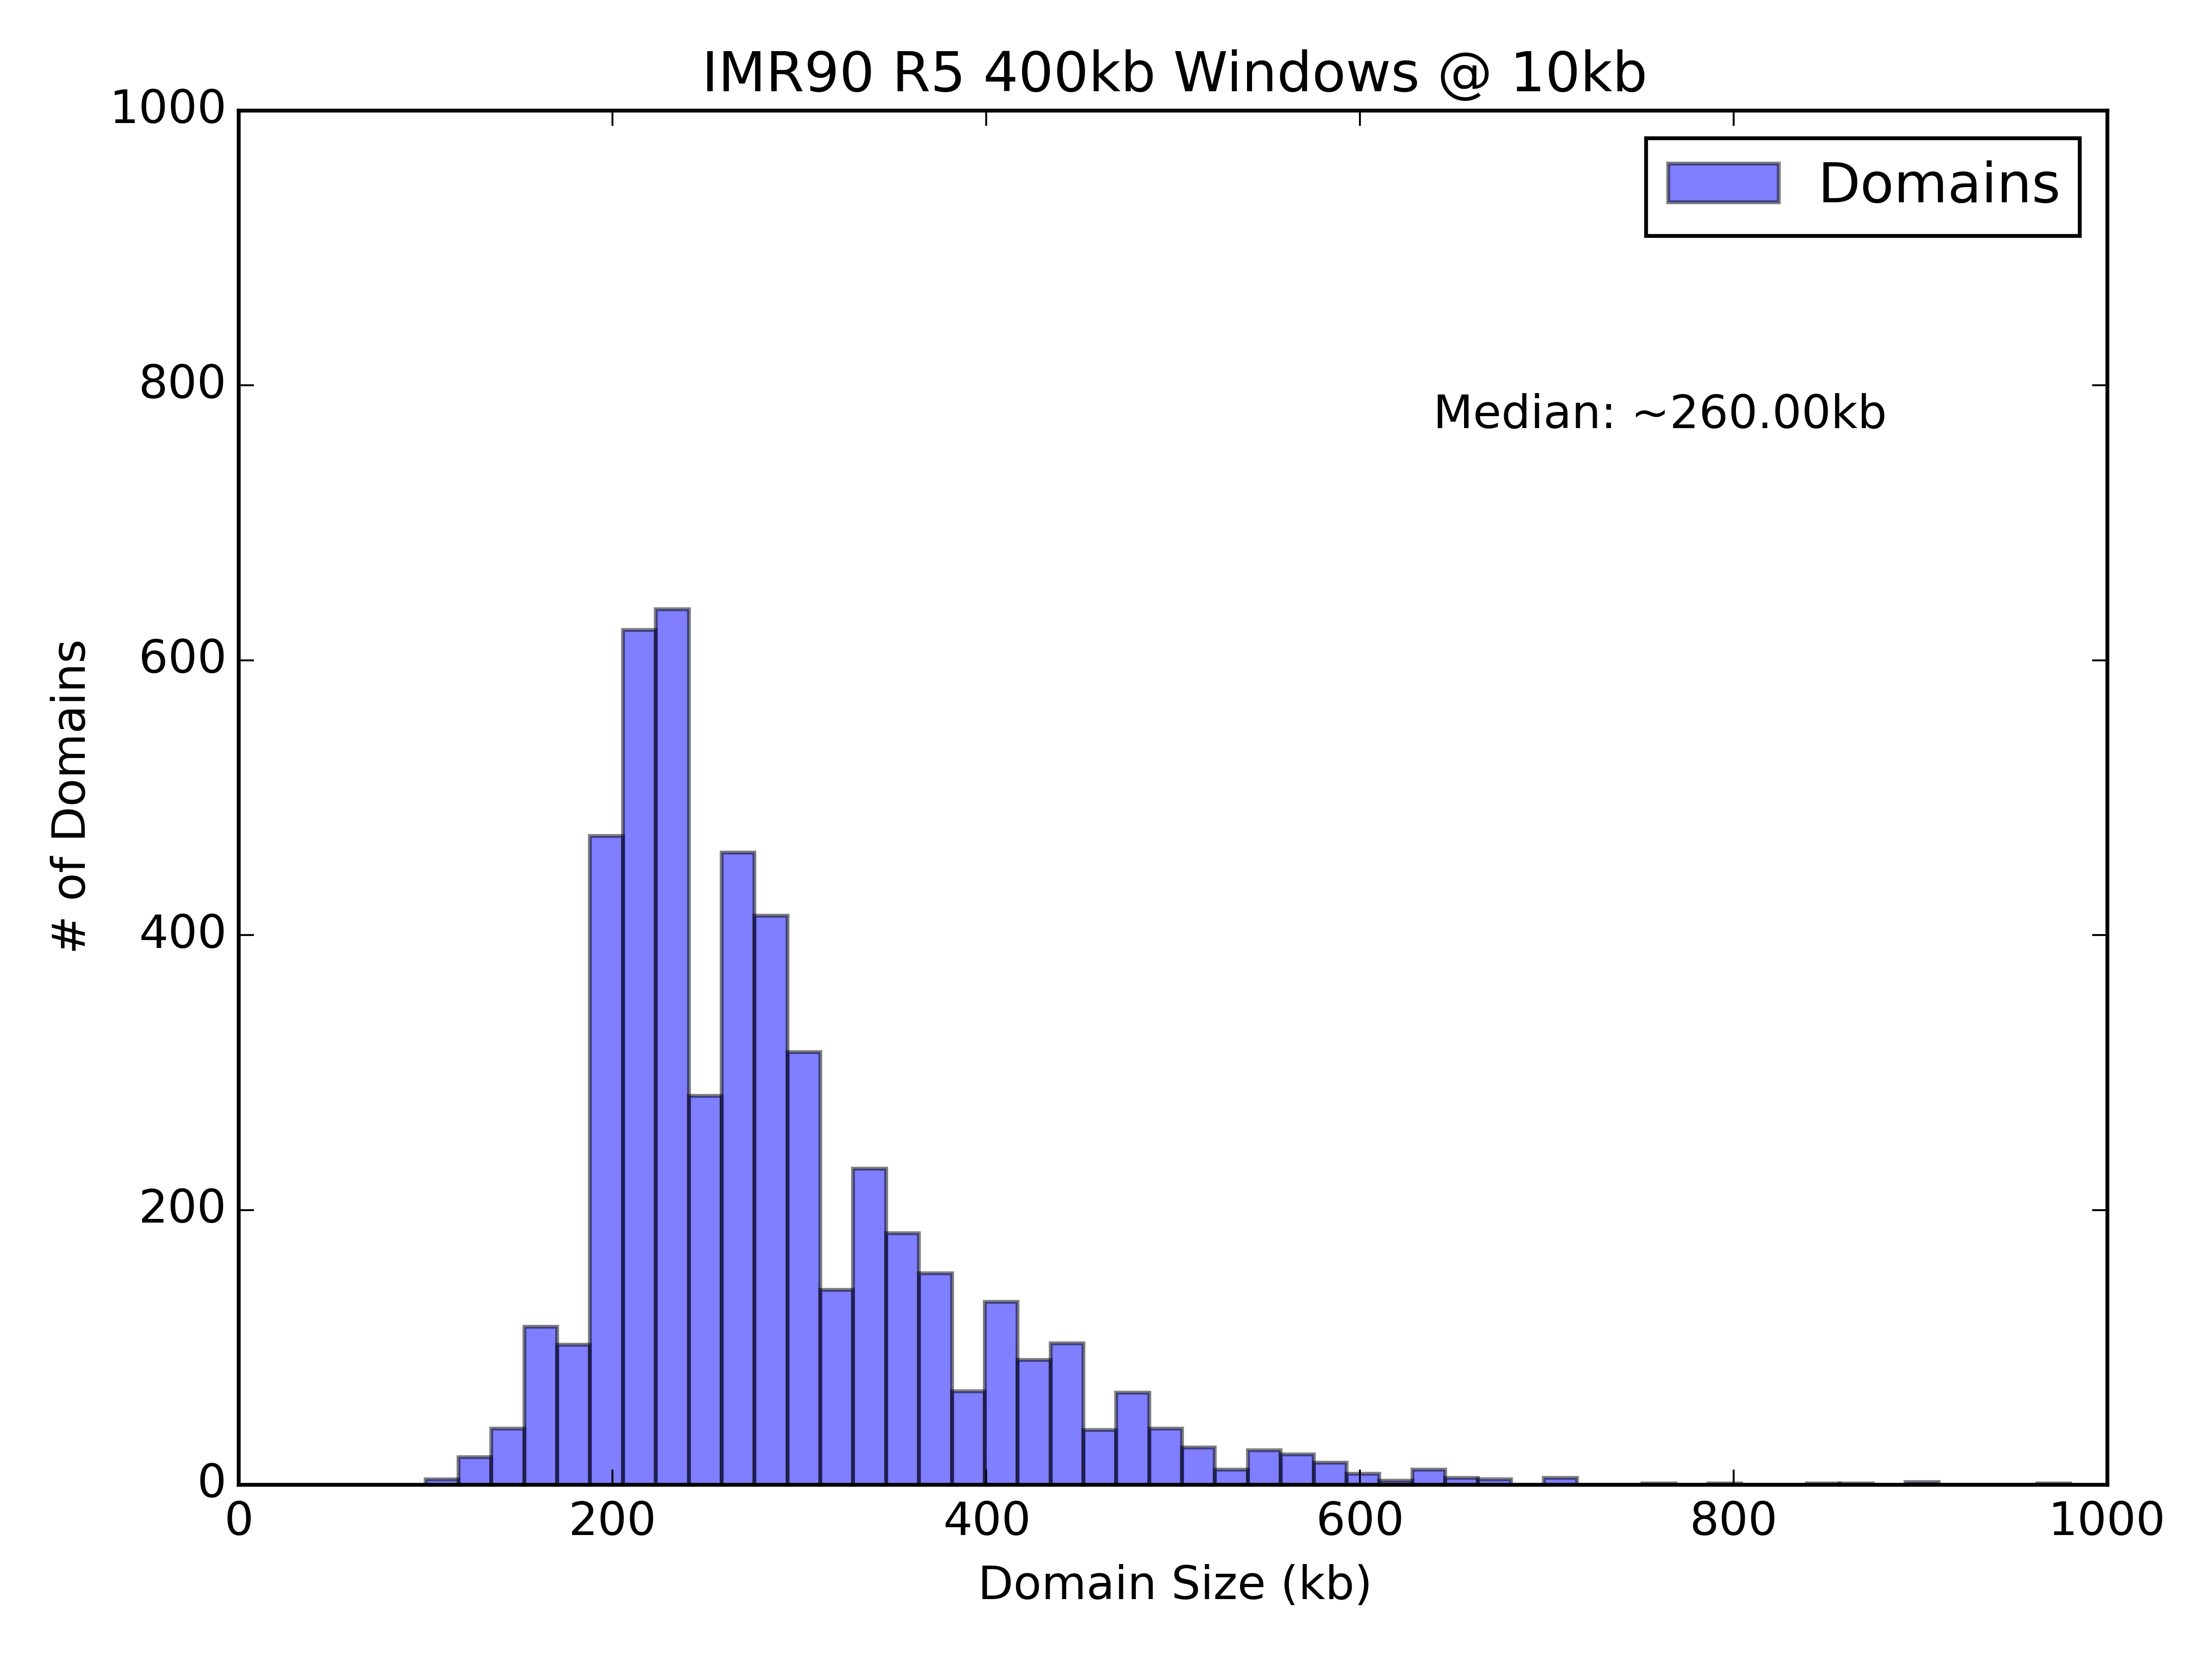
\includegraphics[width=\textwidth]{./figures/supplementary/domains/size400kb.png}
  \end{minipage}%

  \vfill

  \begin{minipage}{0.5\textwidth}%
    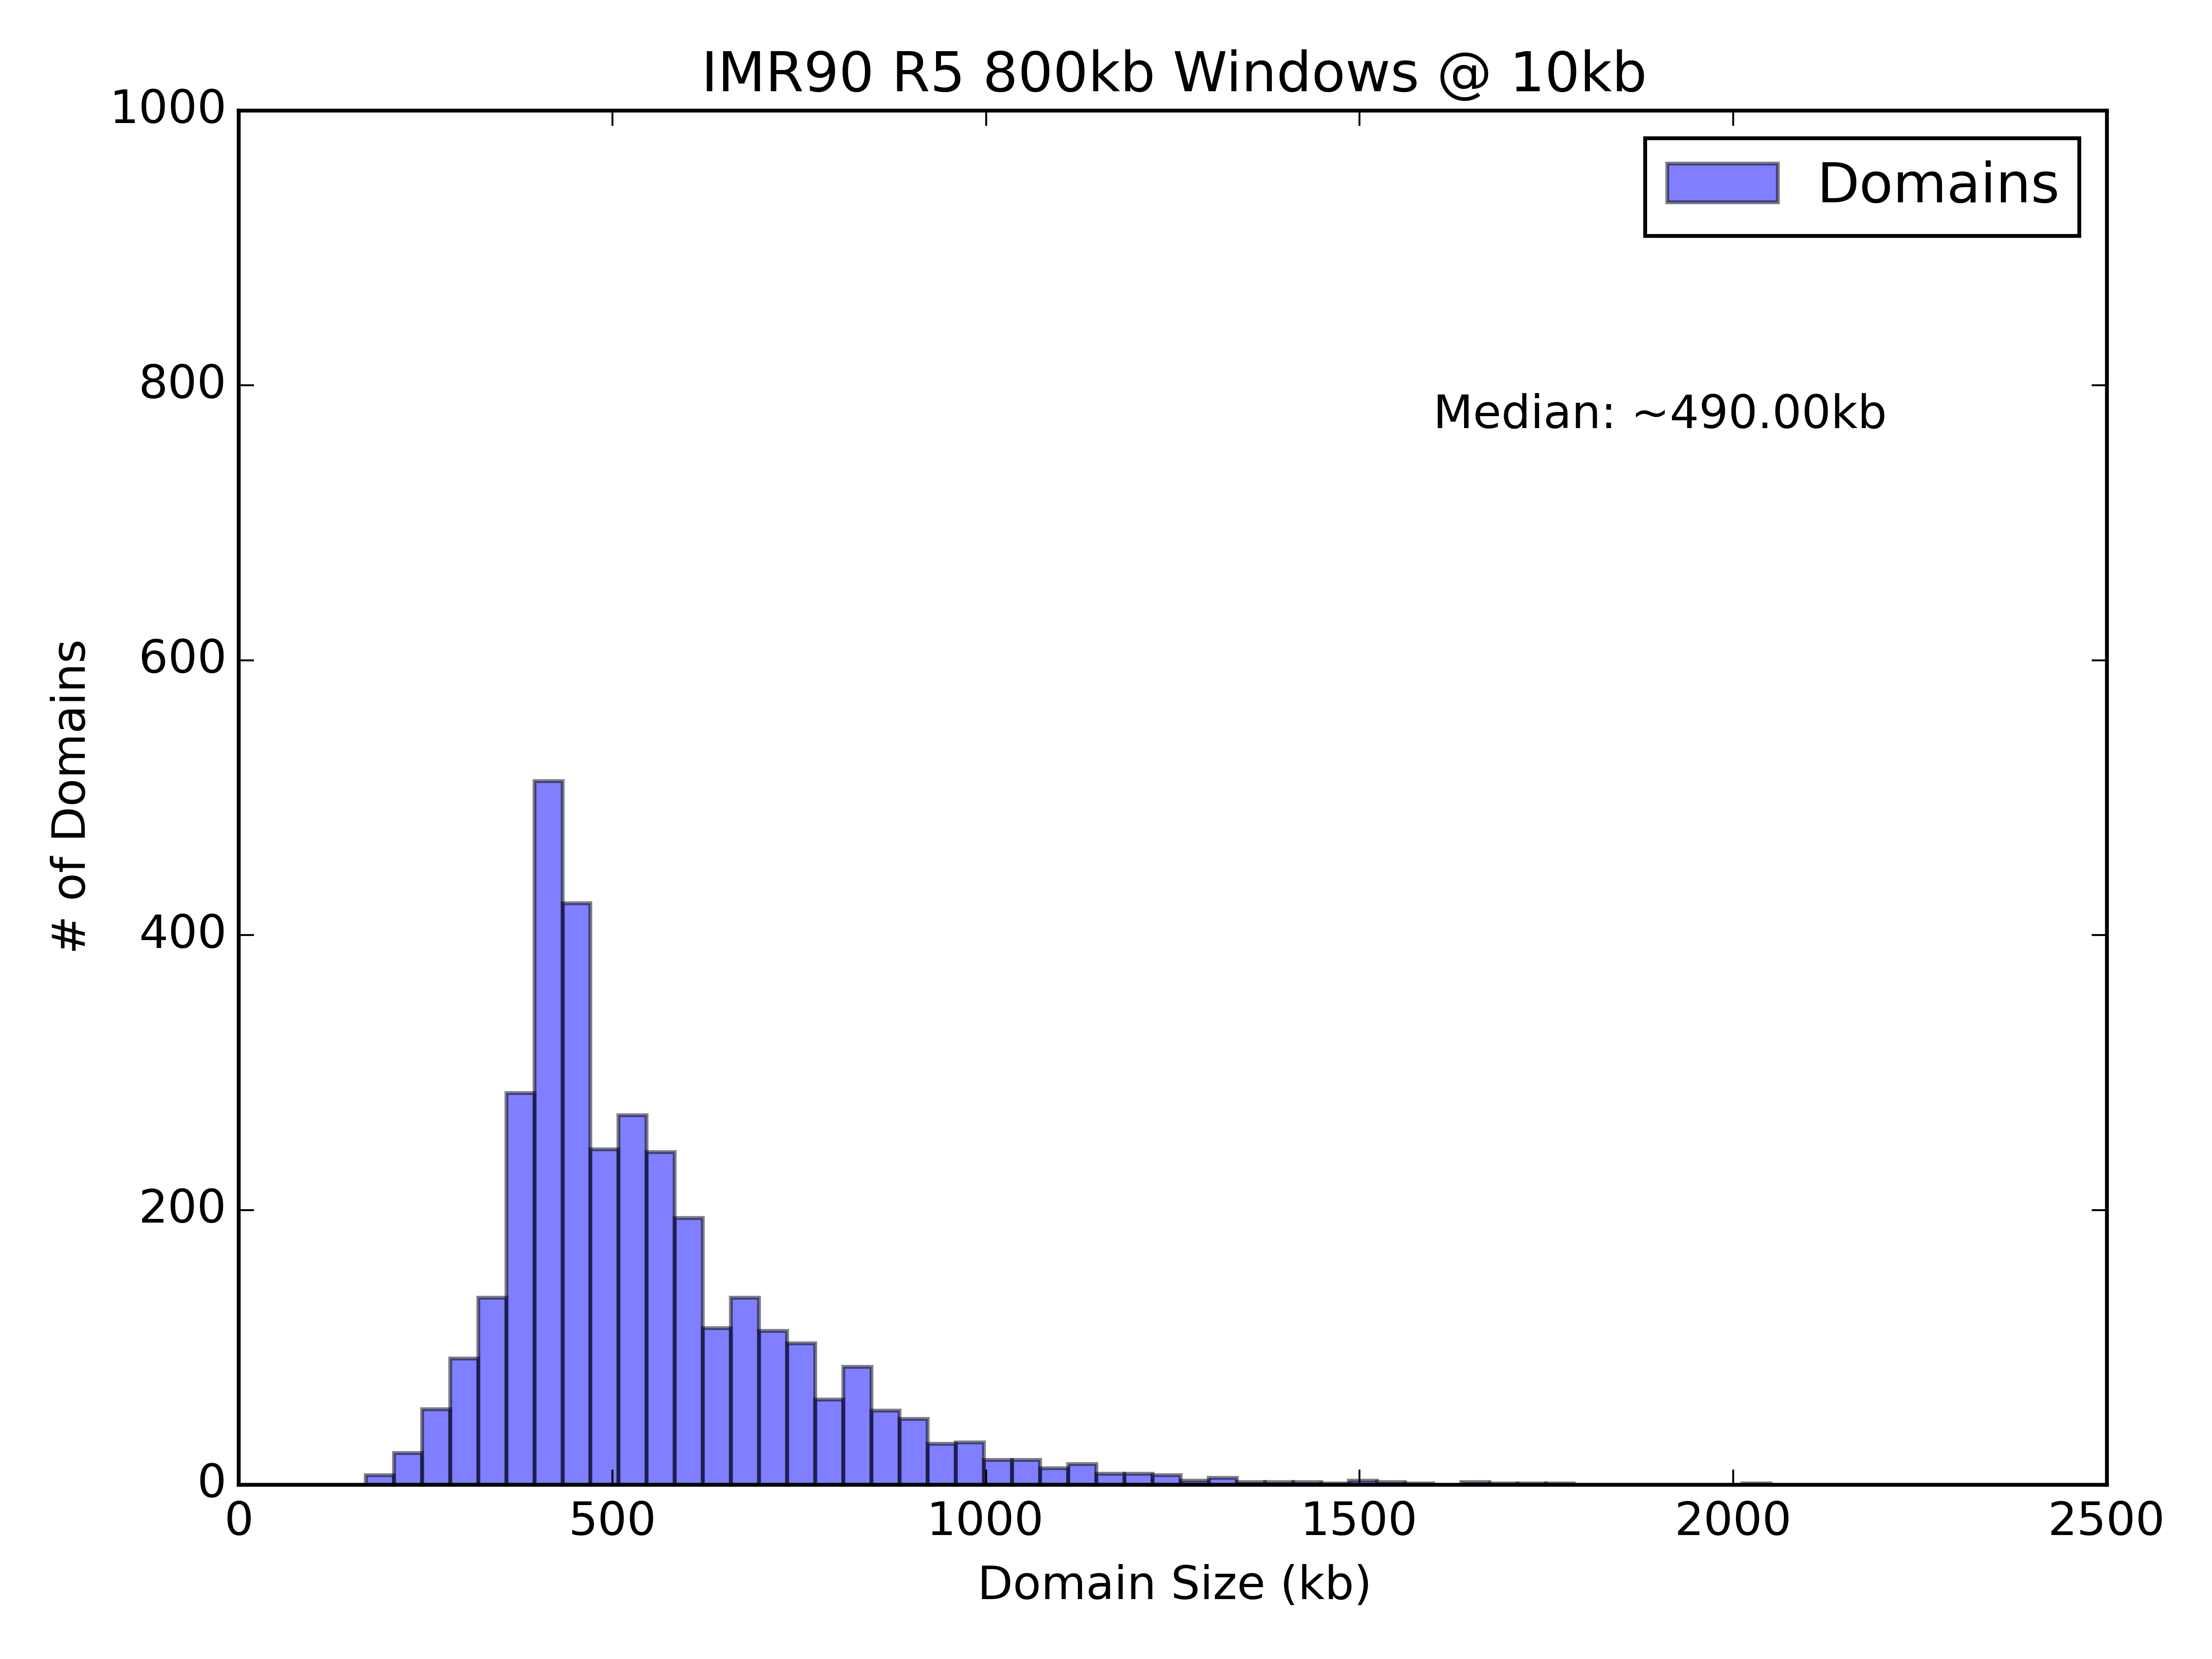
\includegraphics[width=\textwidth]{./figures/supplementary/domains/size800kb.png}
  \end{minipage}%
  \hfill
  \begin{minipage}{0.5\textwidth}
    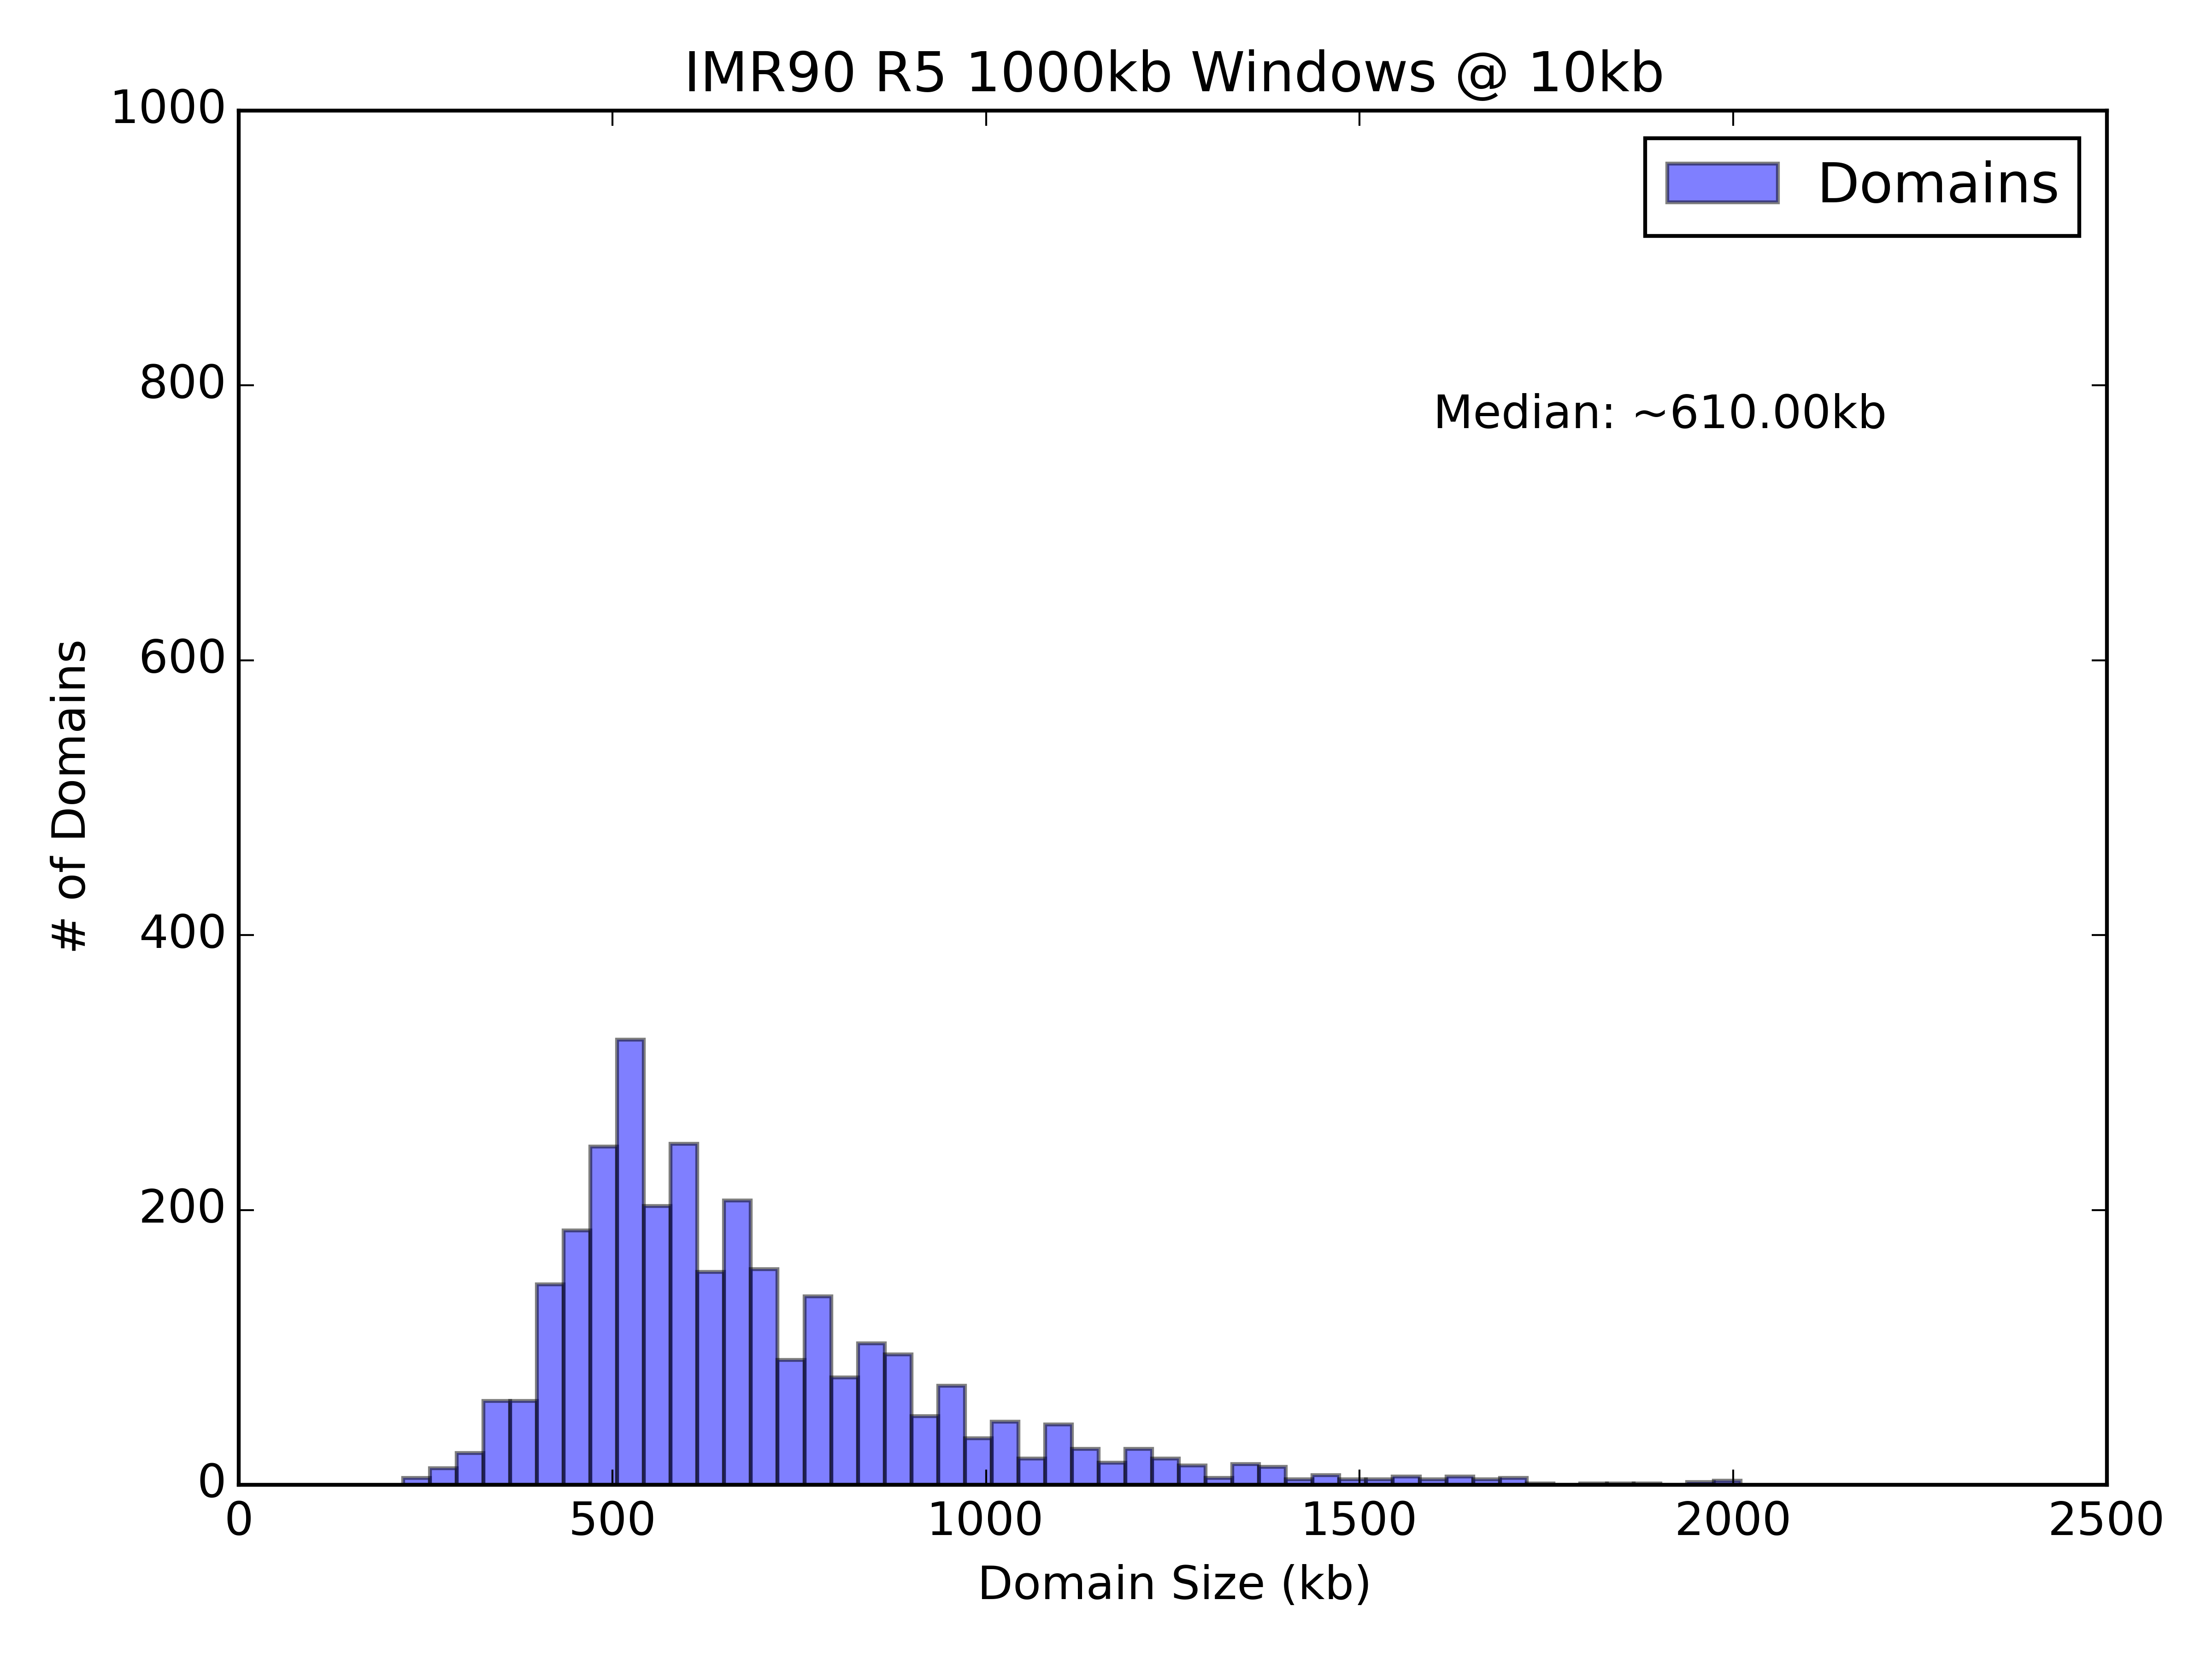
\includegraphics[width=\textwidth]{./figures/supplementary/domains/size1000kb.png}
  \end{minipage}
  \medskip
  \small
  Histogram of domain sizes computed for IMR90 Replicate V.
\end{figure}

\begin{figure}[H]
  \caption{Domain Overlaps by Window Size}
  \begin{minipage}{0.5\textwidth}%
    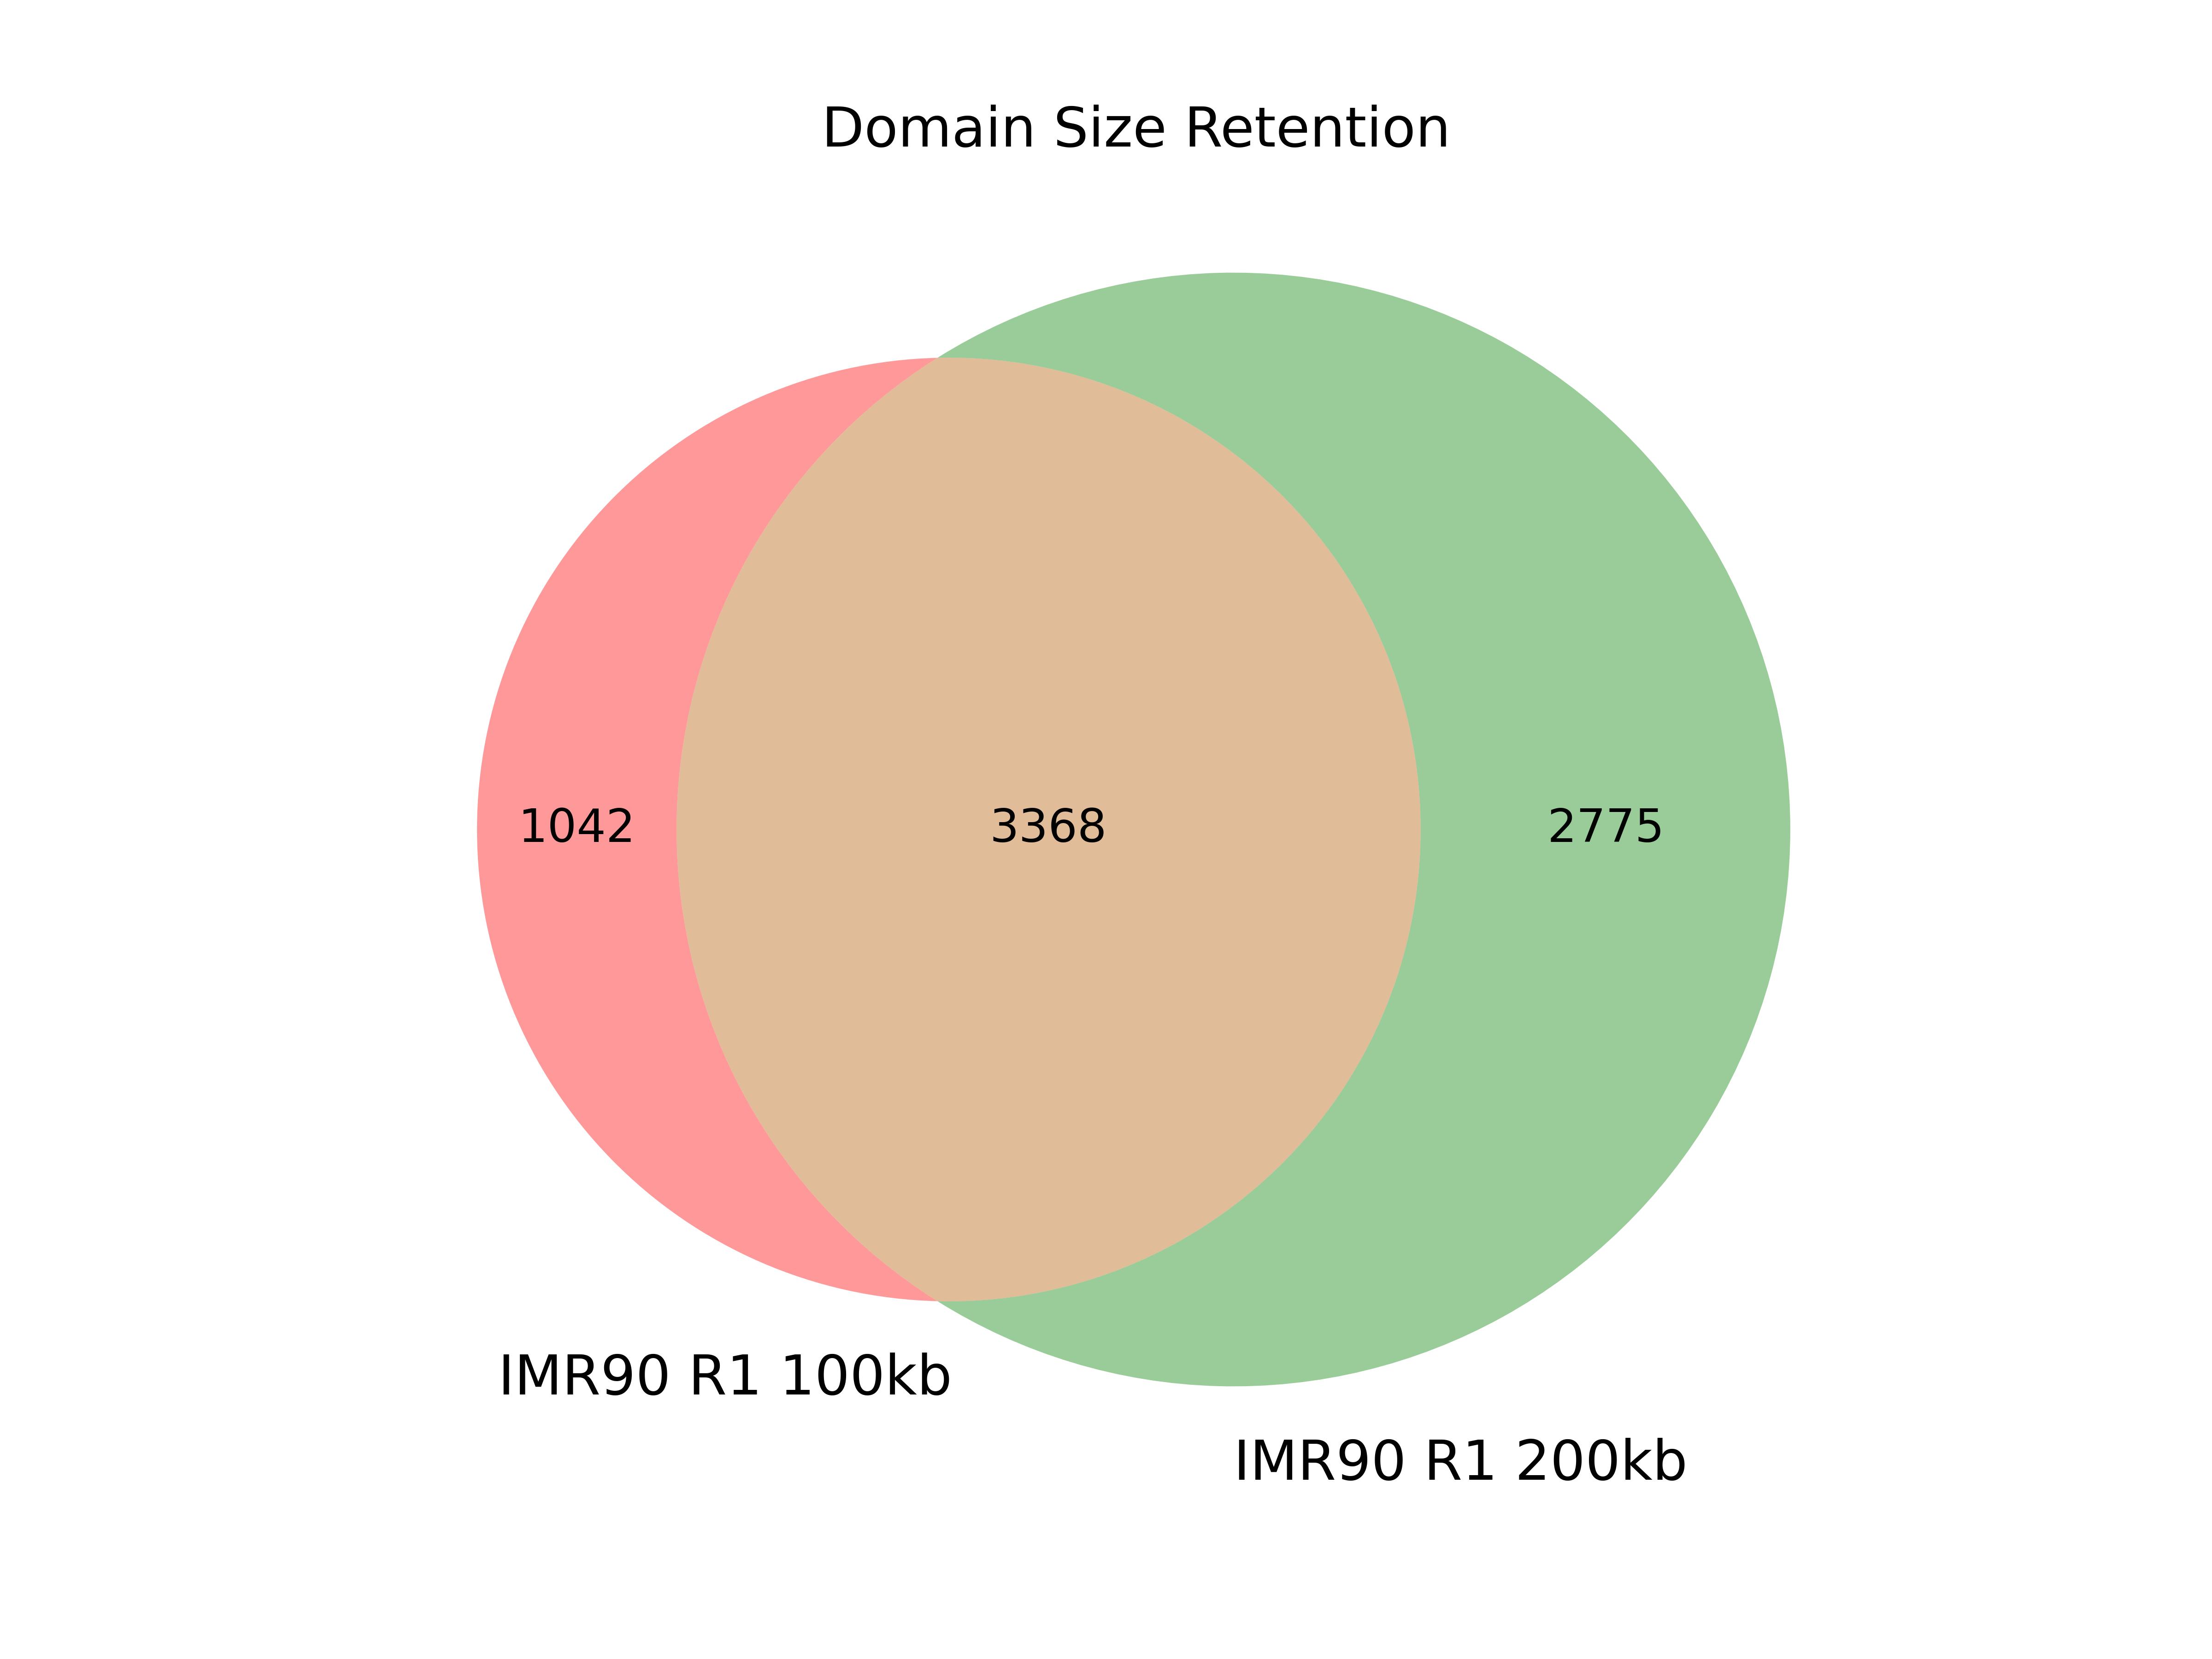
\includegraphics[width=\textwidth]{./figures/supplementary/domains/venn2-IMR90-R1-100-vs-IMR90-R1-200.png}
  \end{minipage}%
  \hfill
  \begin{minipage}{0.5\textwidth}
    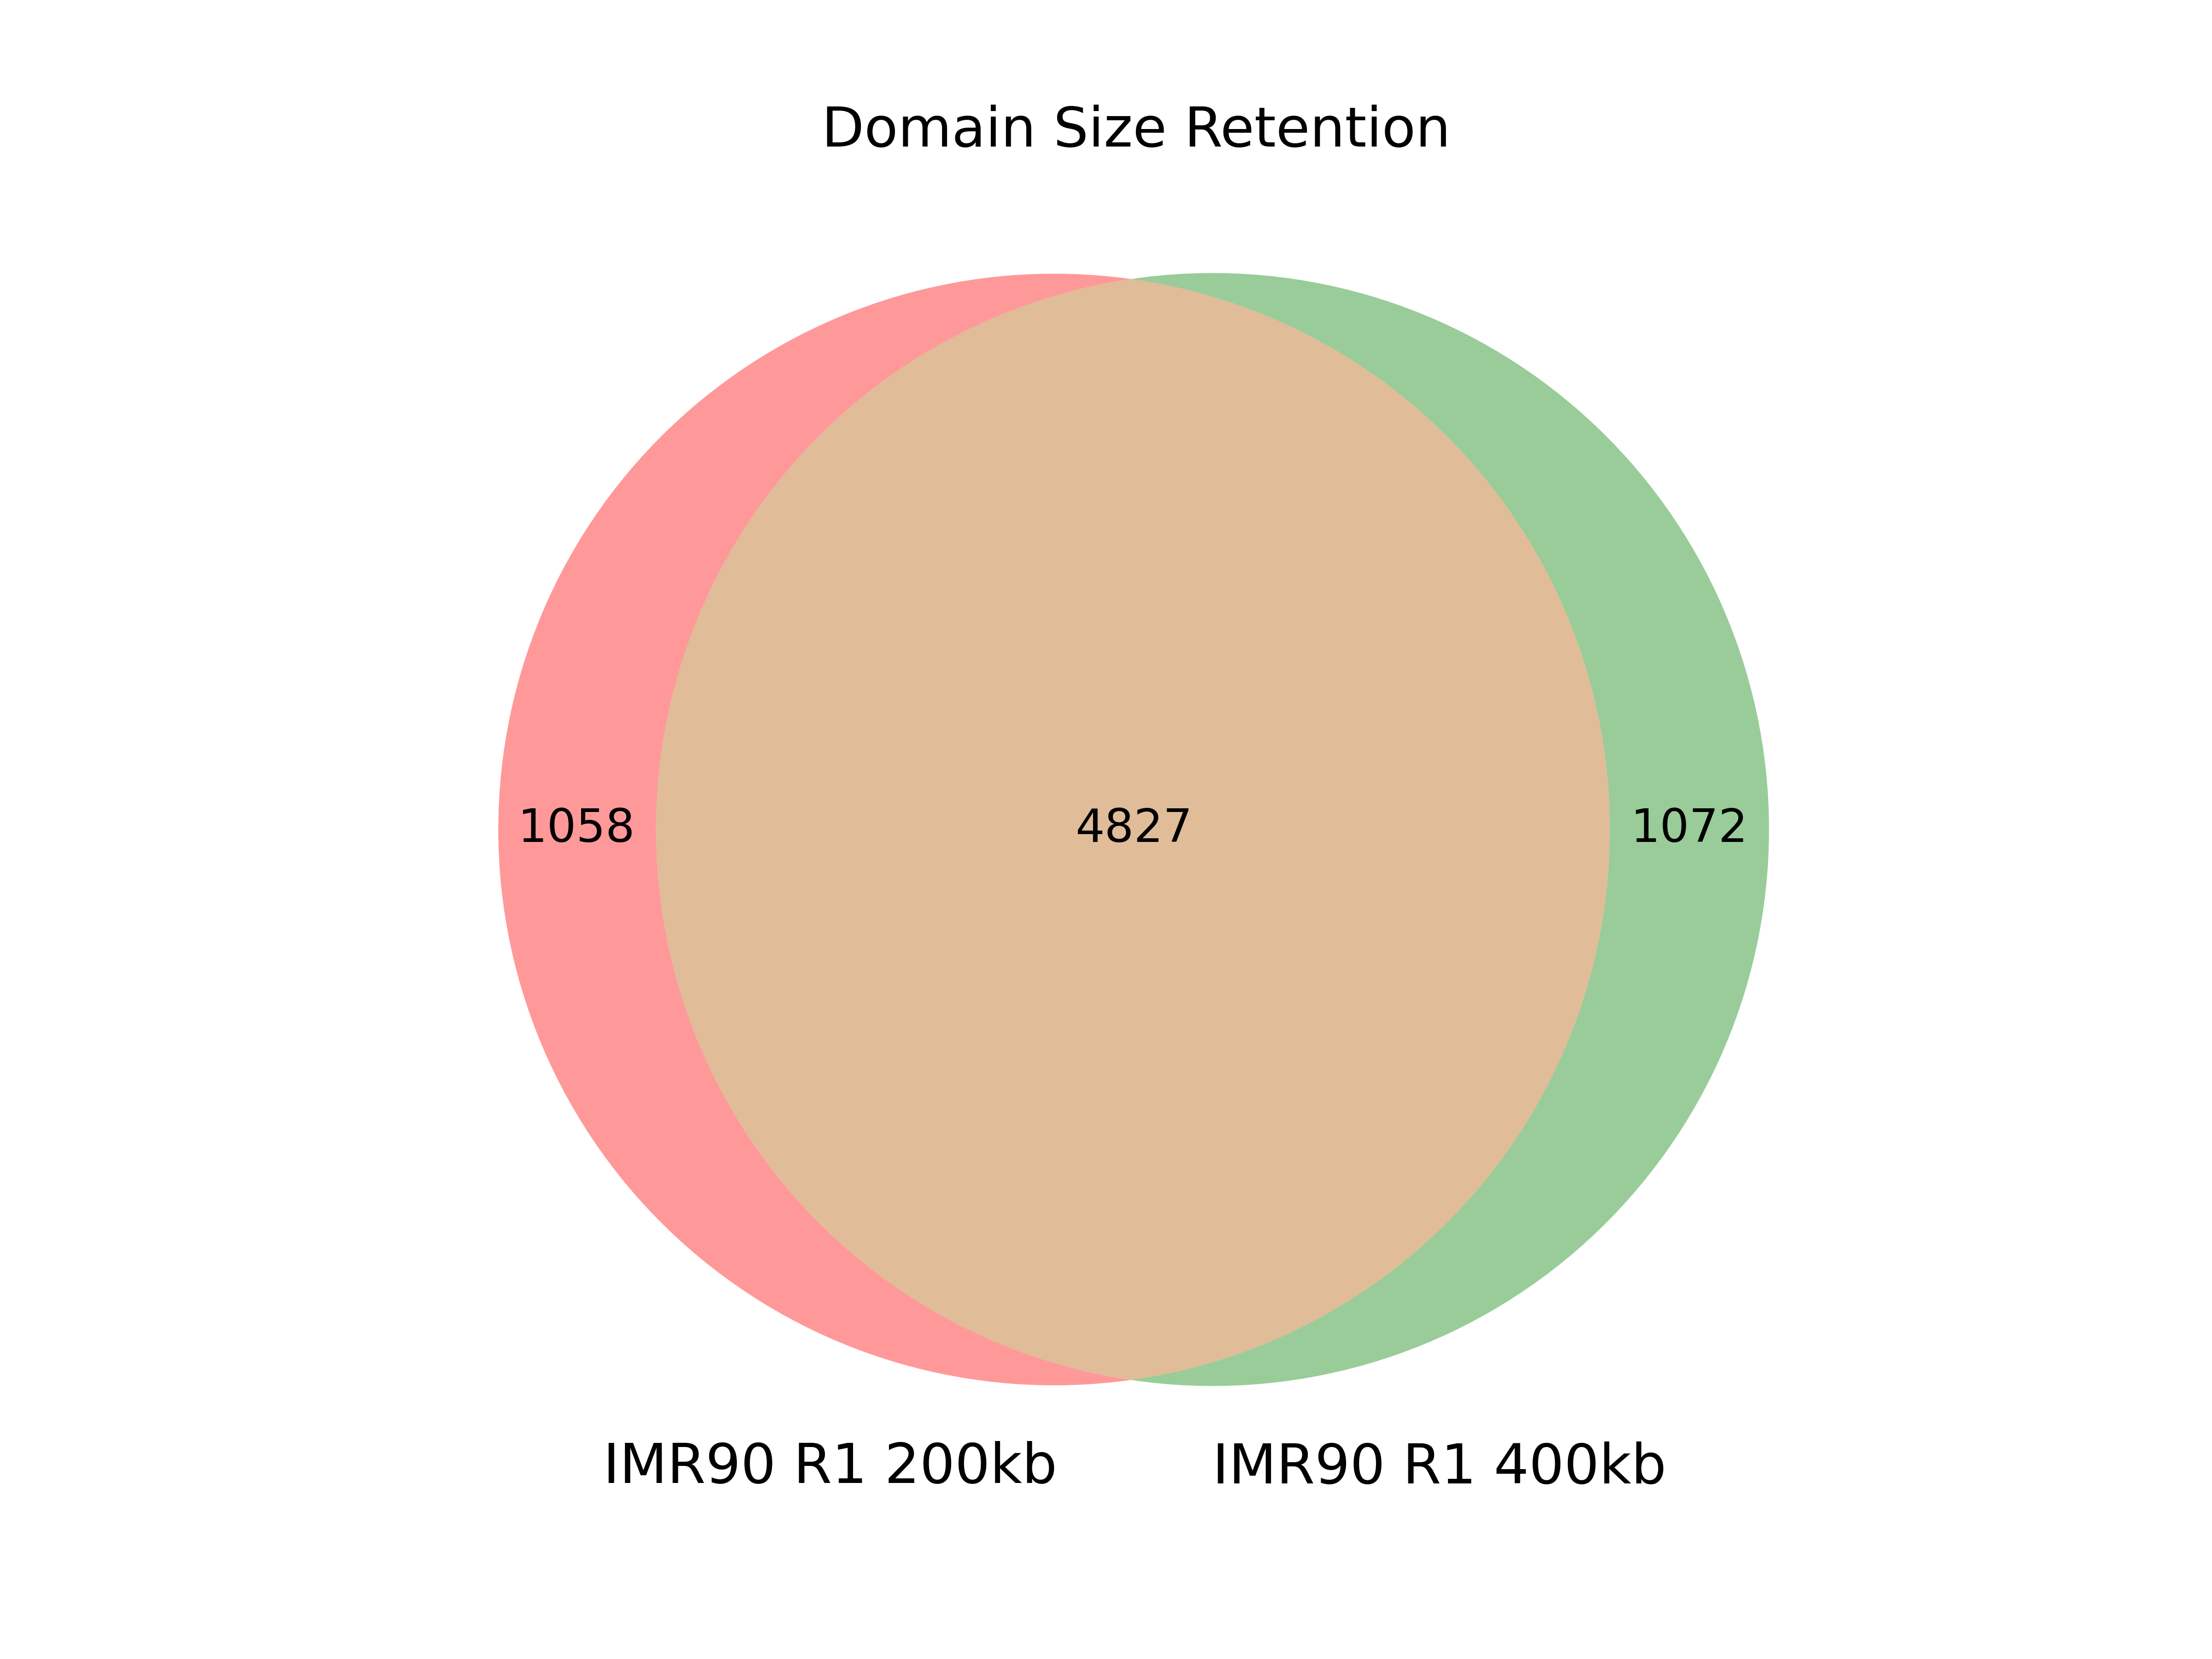
\includegraphics[width=\textwidth]{./figures/supplementary/domains/venn2-IMR90-R1-200-vs-IMR90-R1-400.png}
  \end{minipage}%

  \vfill

  \begin{minipage}{0.5\textwidth}%
    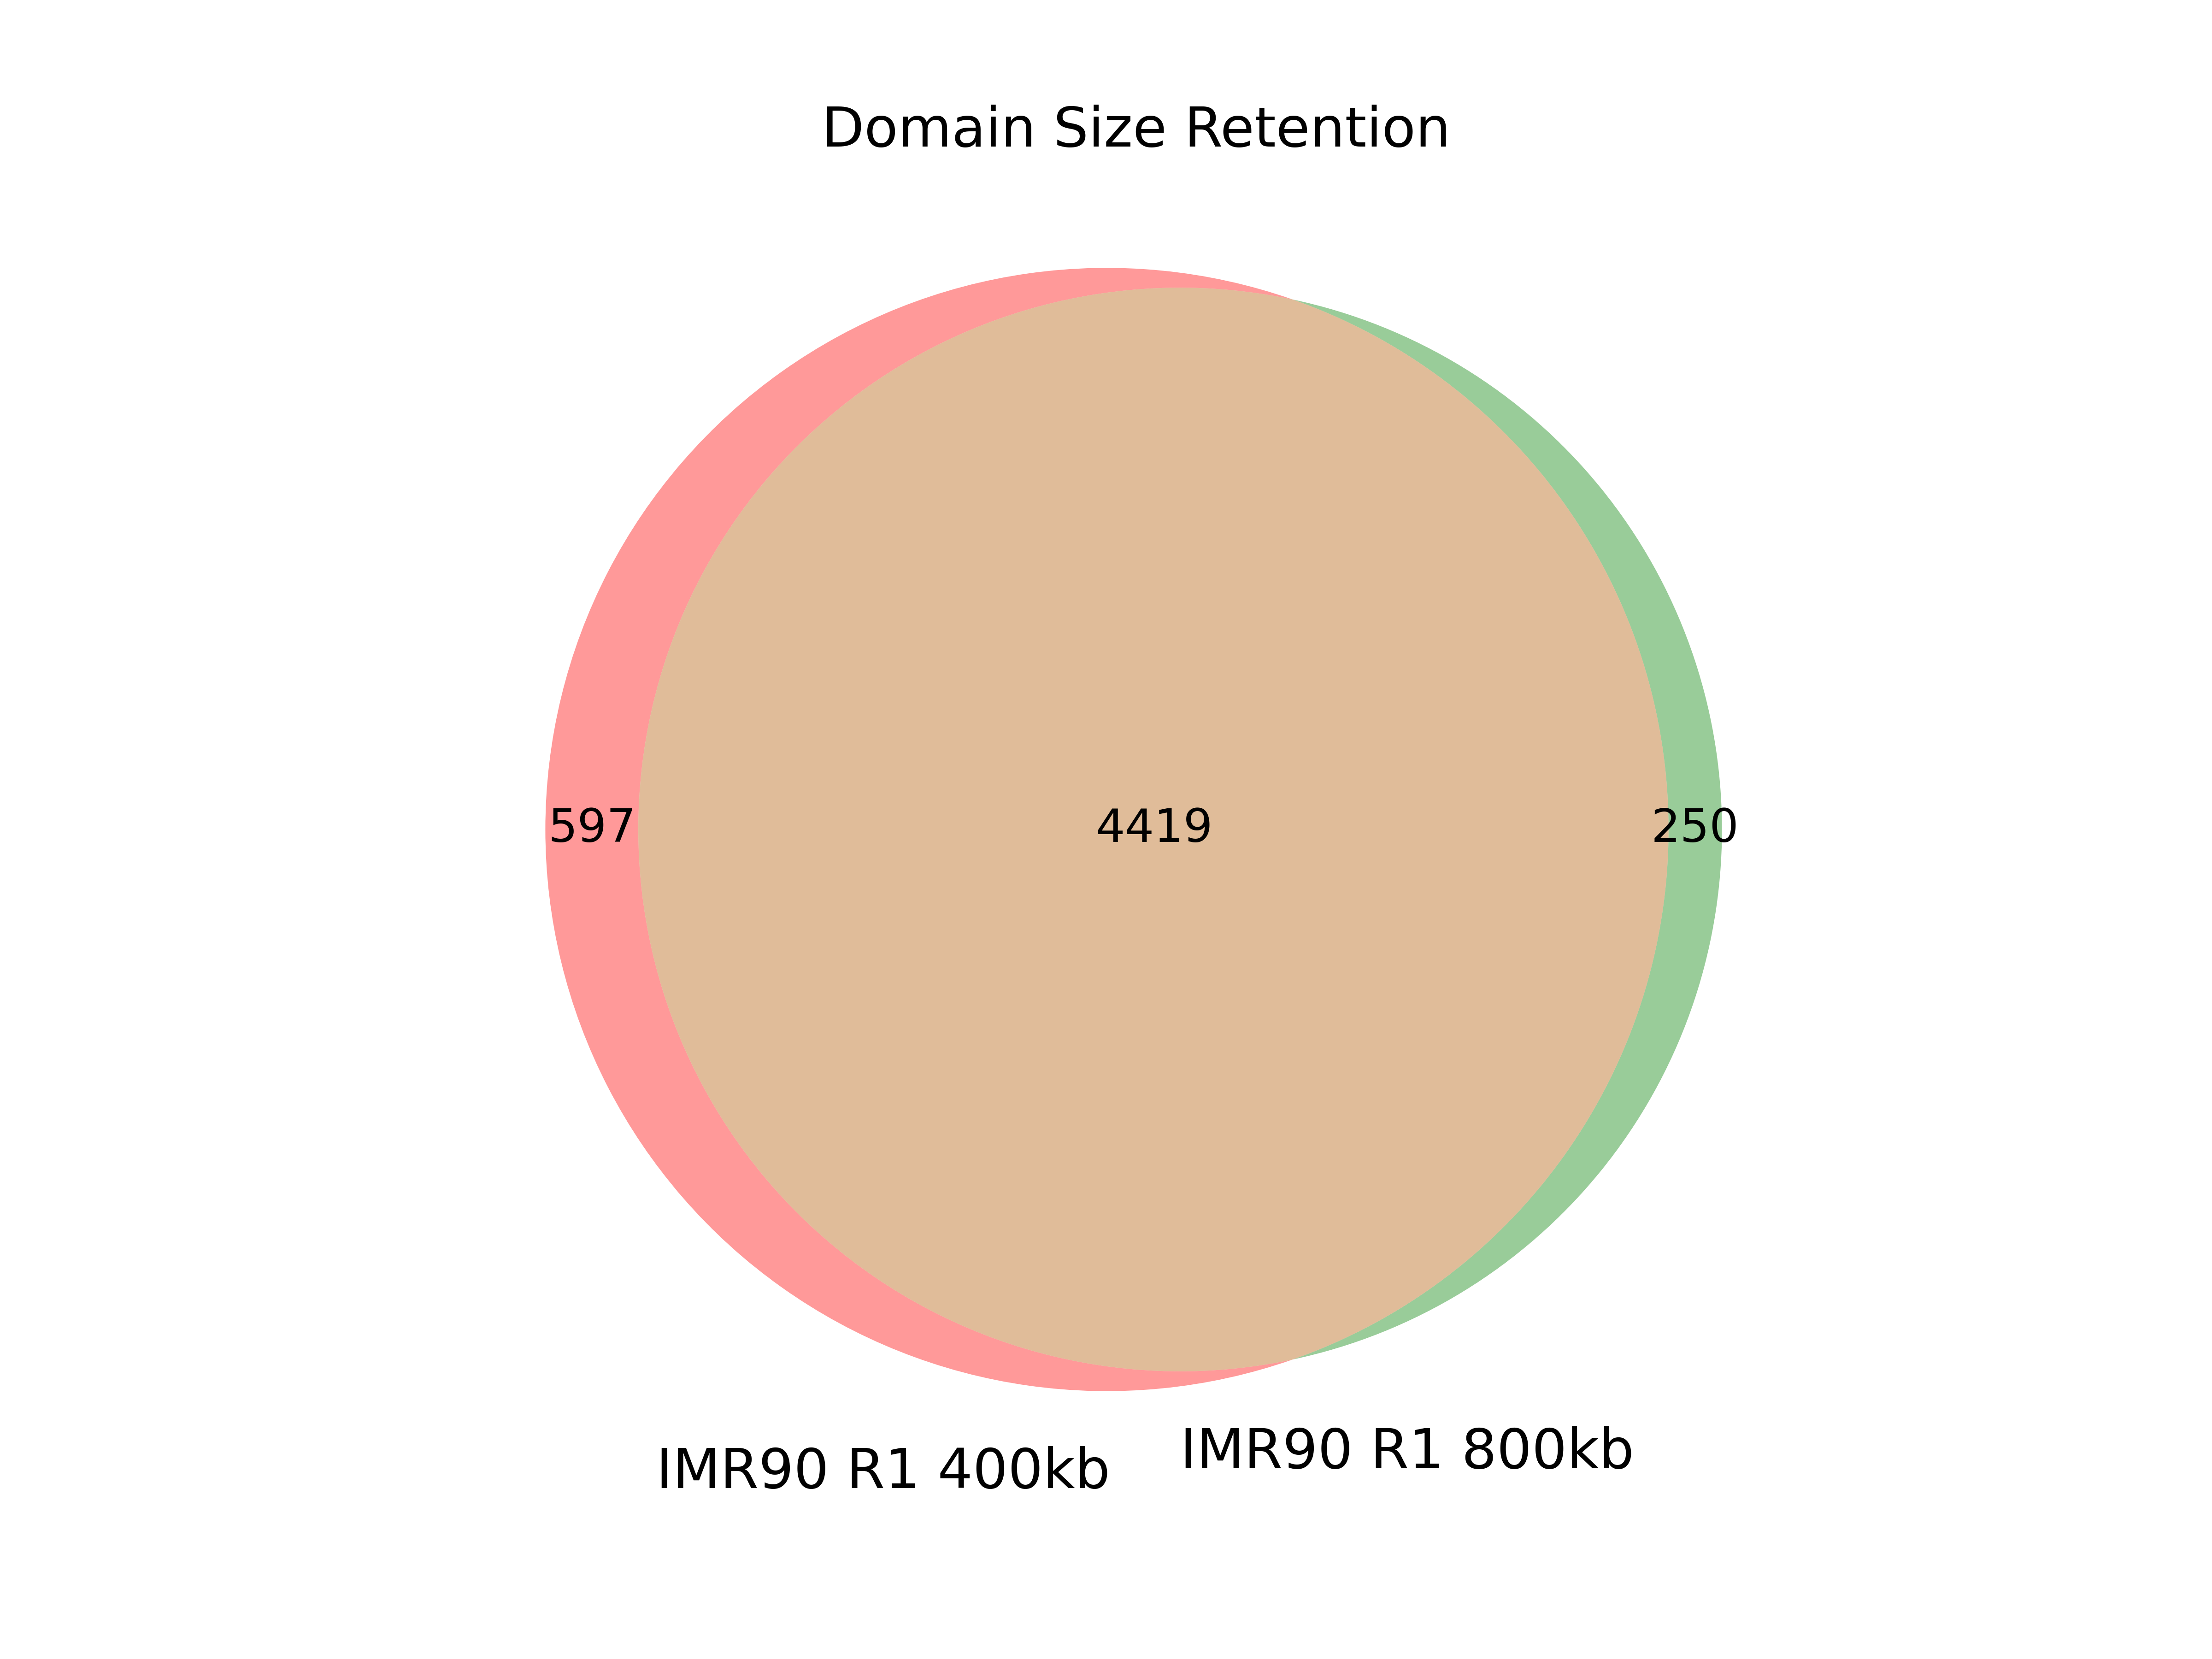
\includegraphics[width=\textwidth]{./figures/supplementary/domains/venn2-IMR90-R1-400-vs-IMR90-R1-800.png}
  \end{minipage}%
  \hfill
  \begin{minipage}{0.5\textwidth}
    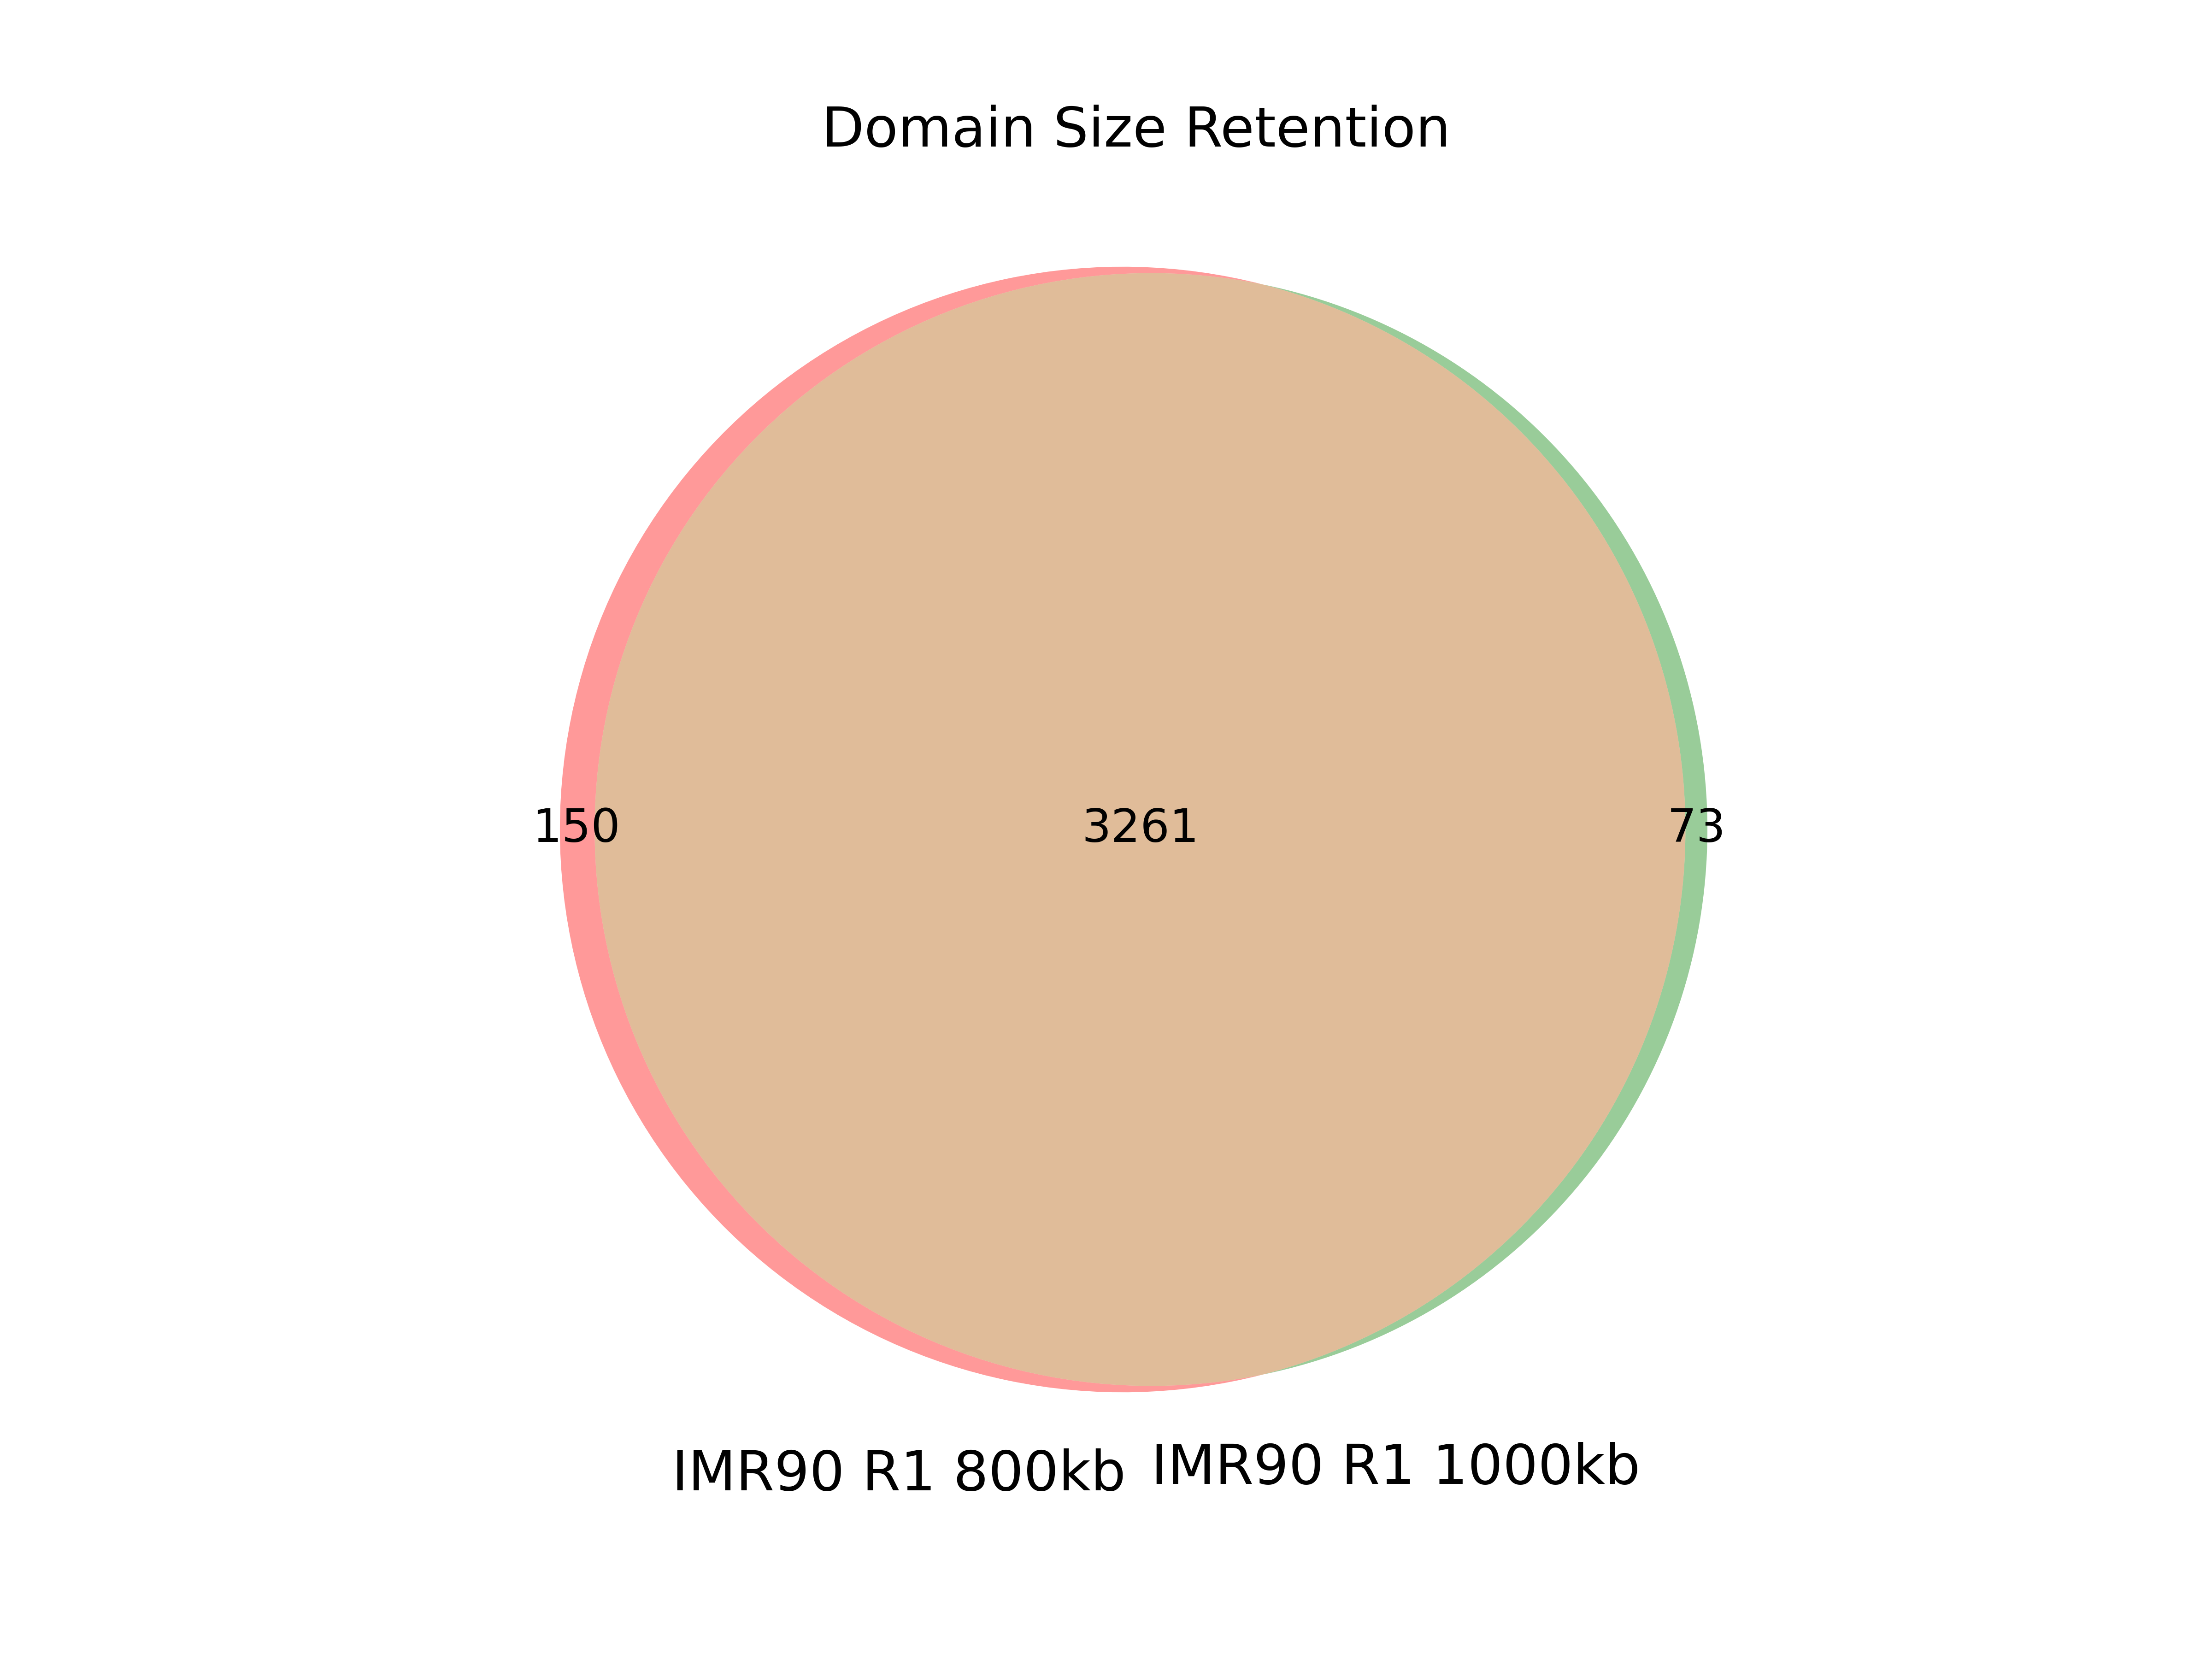
\includegraphics[width=\textwidth]{./figures/supplementary/domains/venn2-IMR90-R1-800-vs-IMR90-R1-1000.png}
  \end{minipage}
  \medskip
  \small
  Venn diagrams illustrating overlaps between domains discovered at increasing window sizes.  In general, the
  increasing window size led to increasingly larger domains.  Larger domains often subsumed domains discovered
  with a smaller window size.
\end{figure}

\newpage
\subsection*{Domain Overlaps with Lesions}

\begin{figure}[H]
  \caption{Lesion Overlaps by Window Size}
  \begin{minipage}{0.5\textwidth}%
    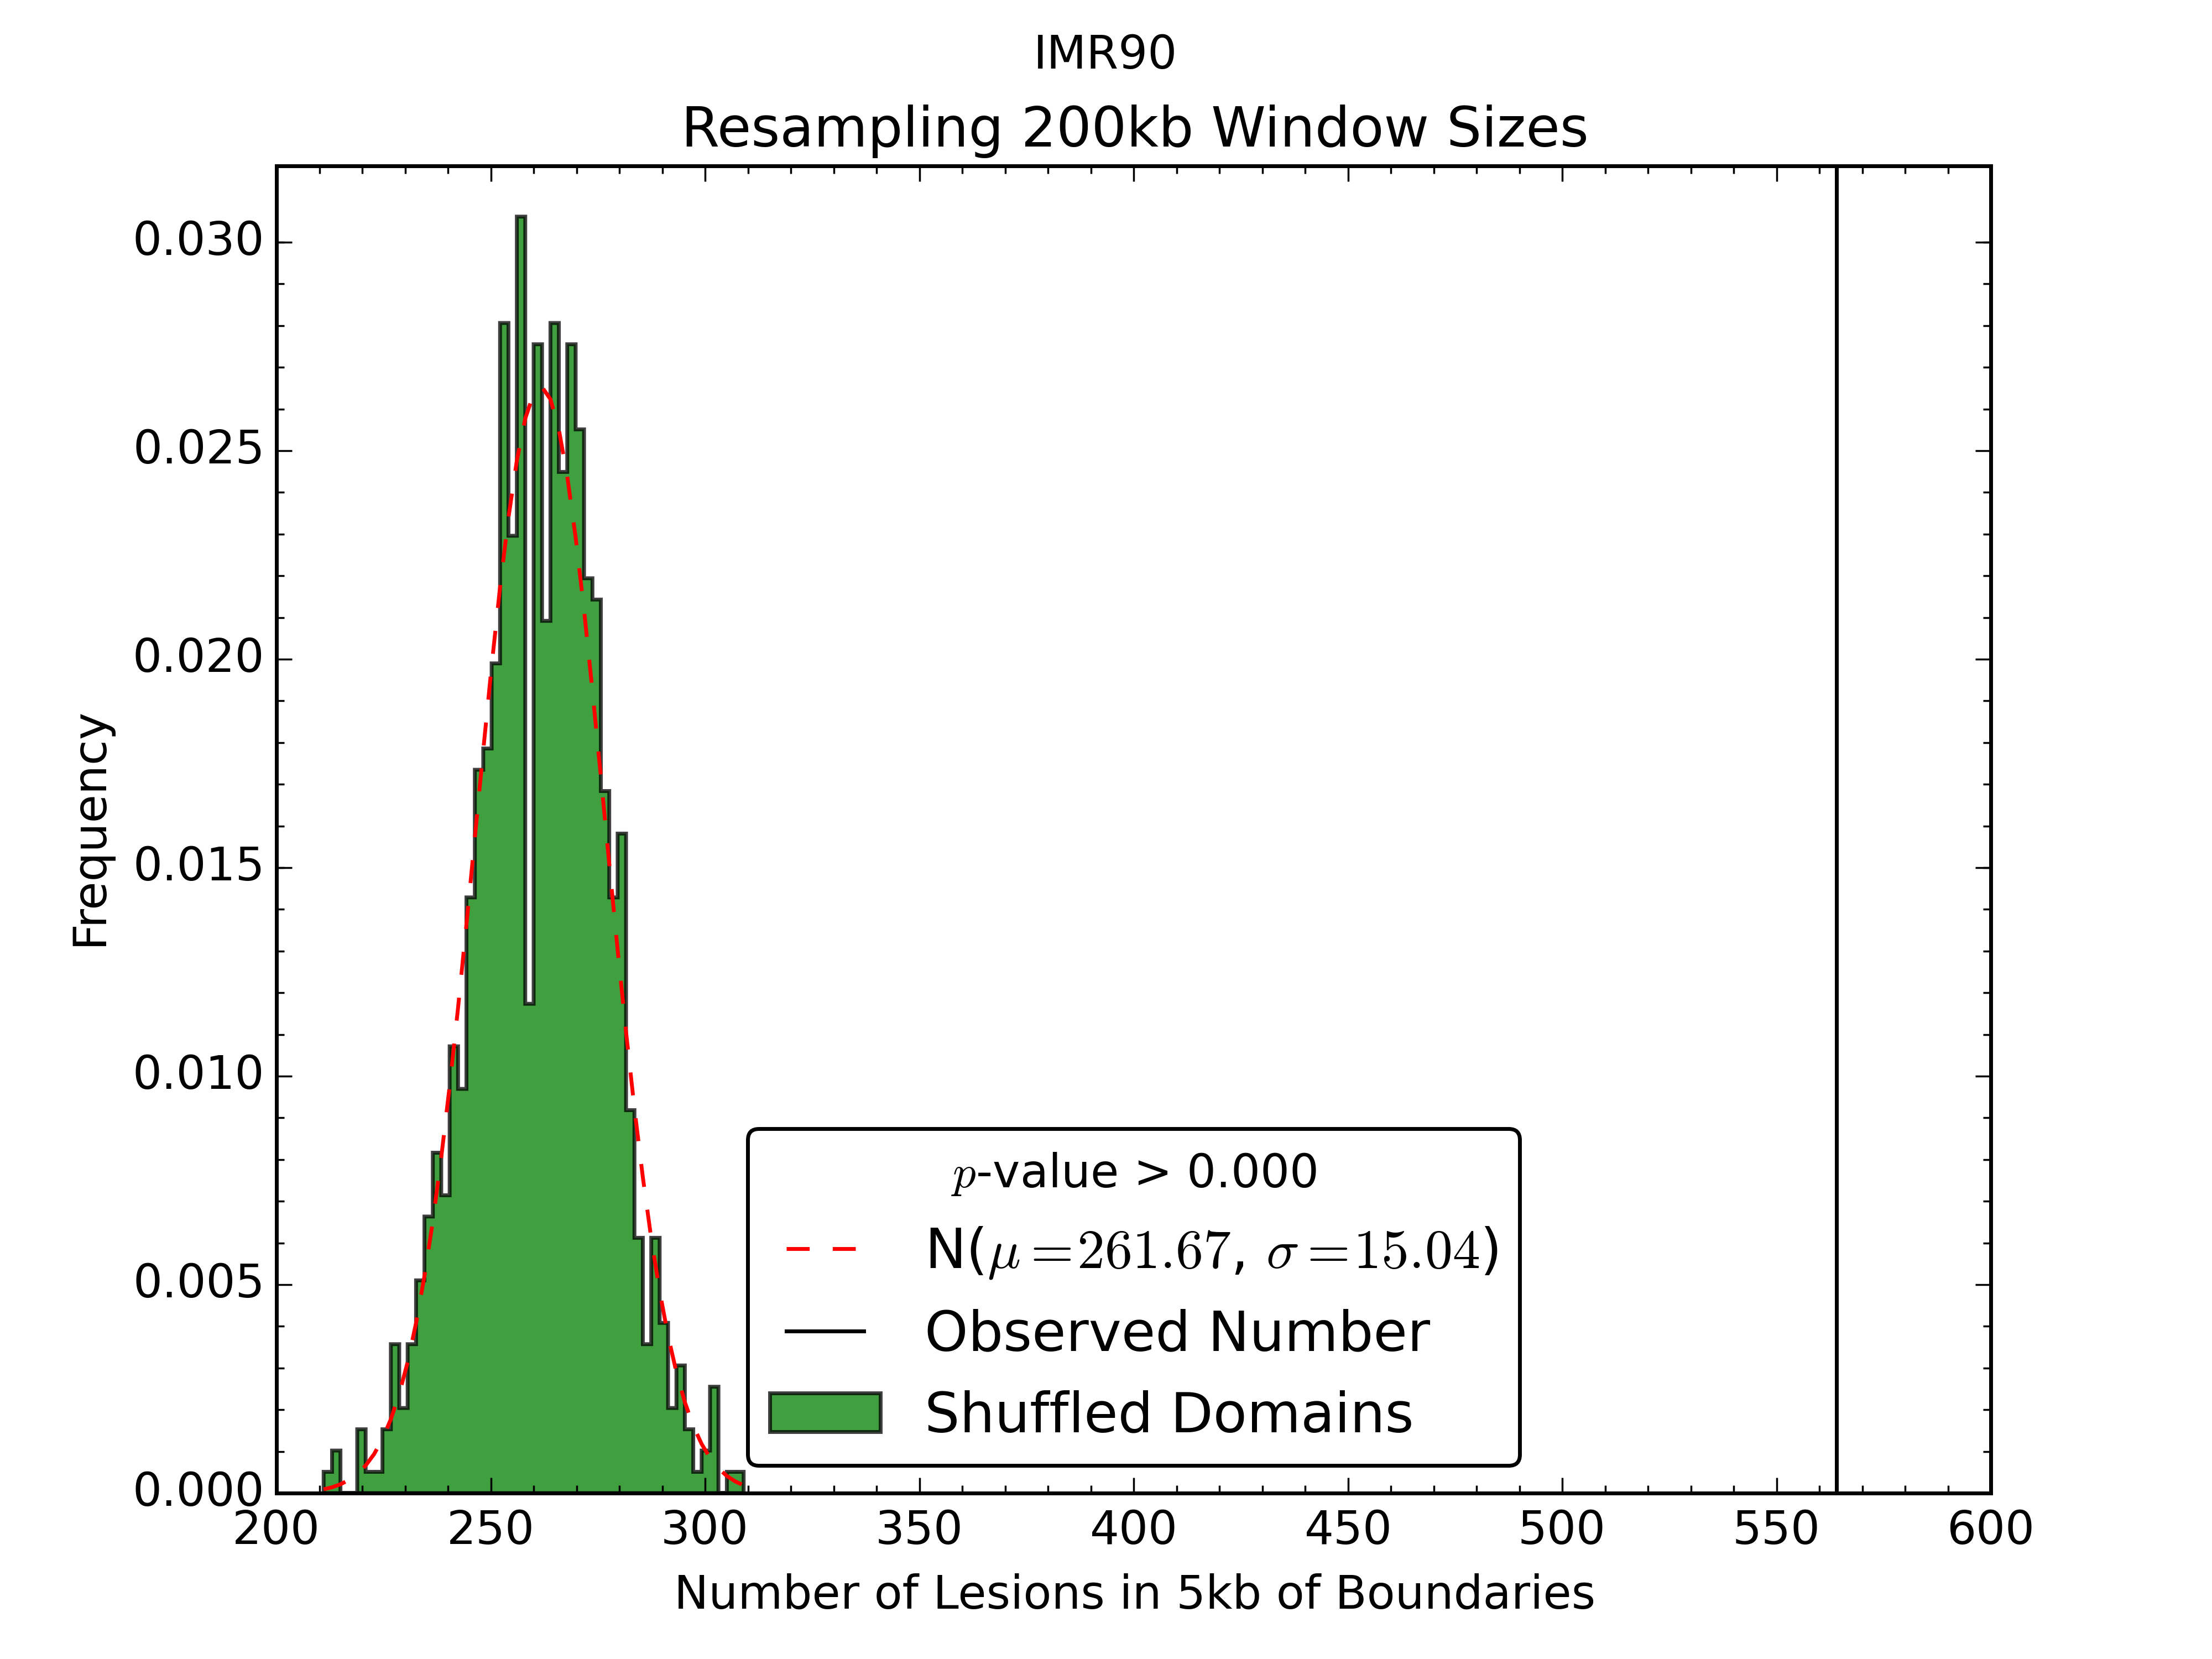
\includegraphics[width=\textwidth]{./figures/supplementary/domains/boundaries-IMR90-200kb.png}
  \end{minipage}%
  \hfill
  \begin{minipage}{0.5\textwidth}
    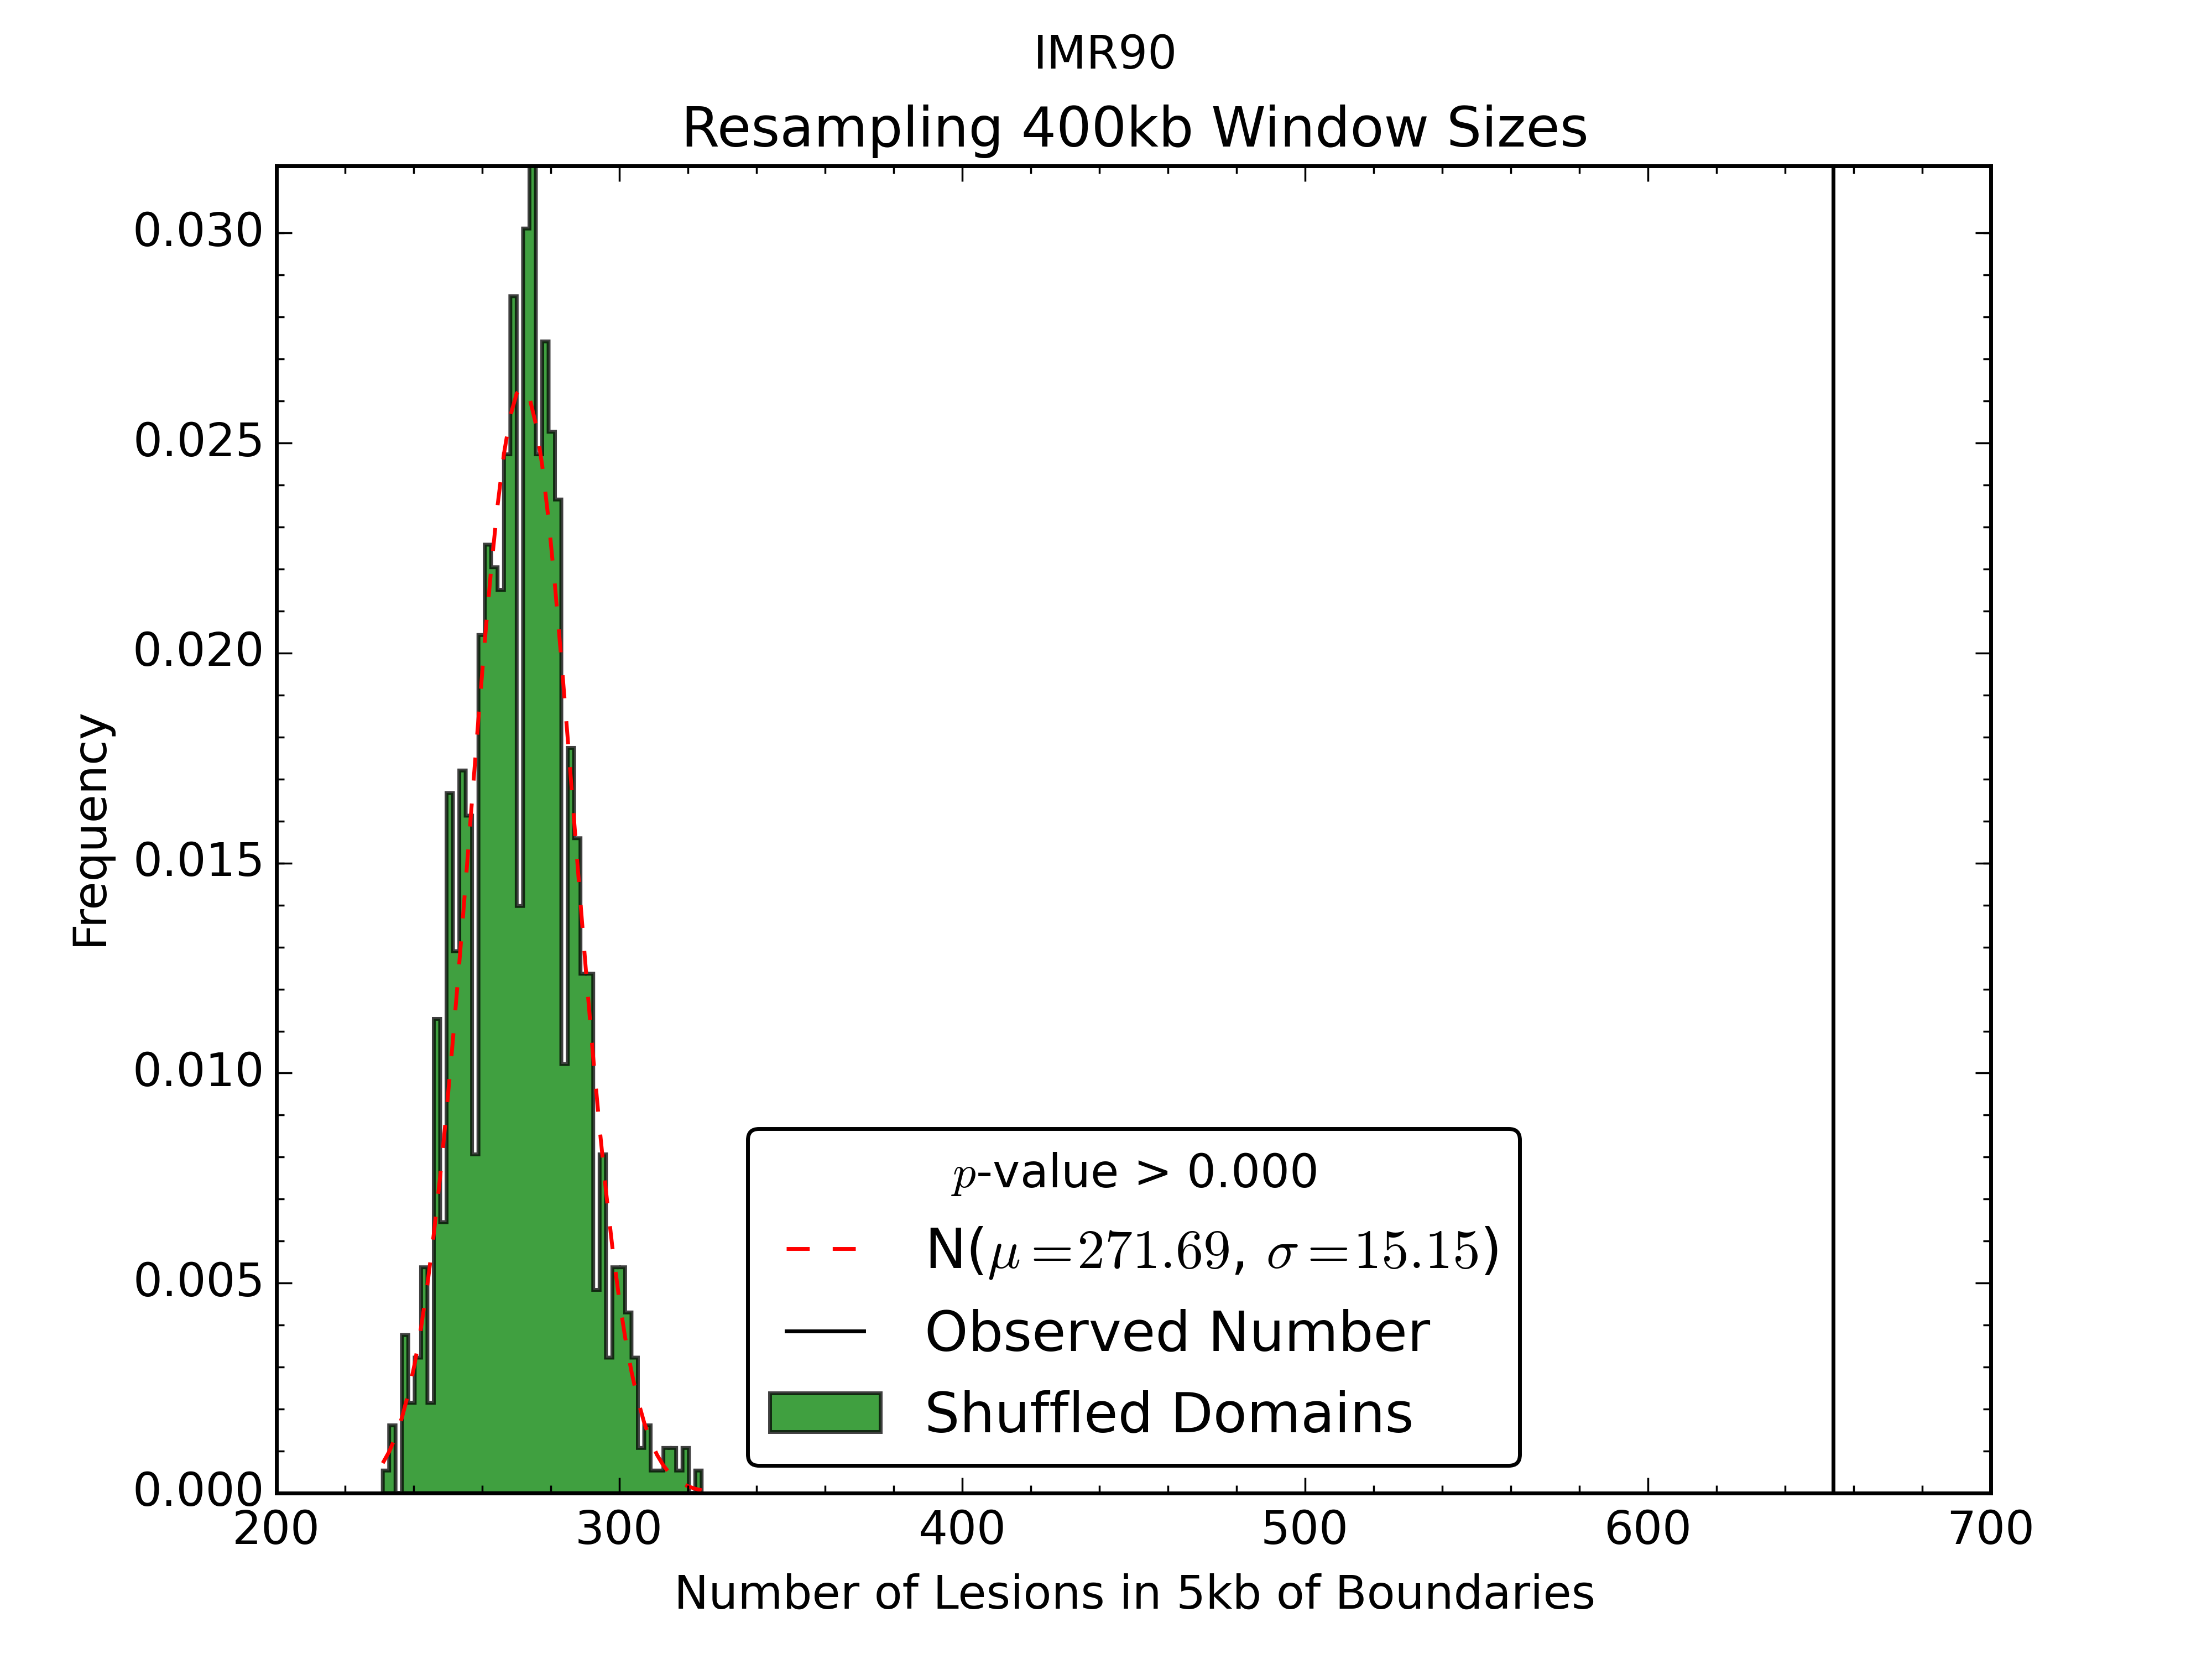
\includegraphics[width=\textwidth]{./figures/supplementary/domains/boundaries-IMR90-400kb.png}
  \end{minipage}%

  \vfill

  \begin{minipage}{0.5\textwidth}%
    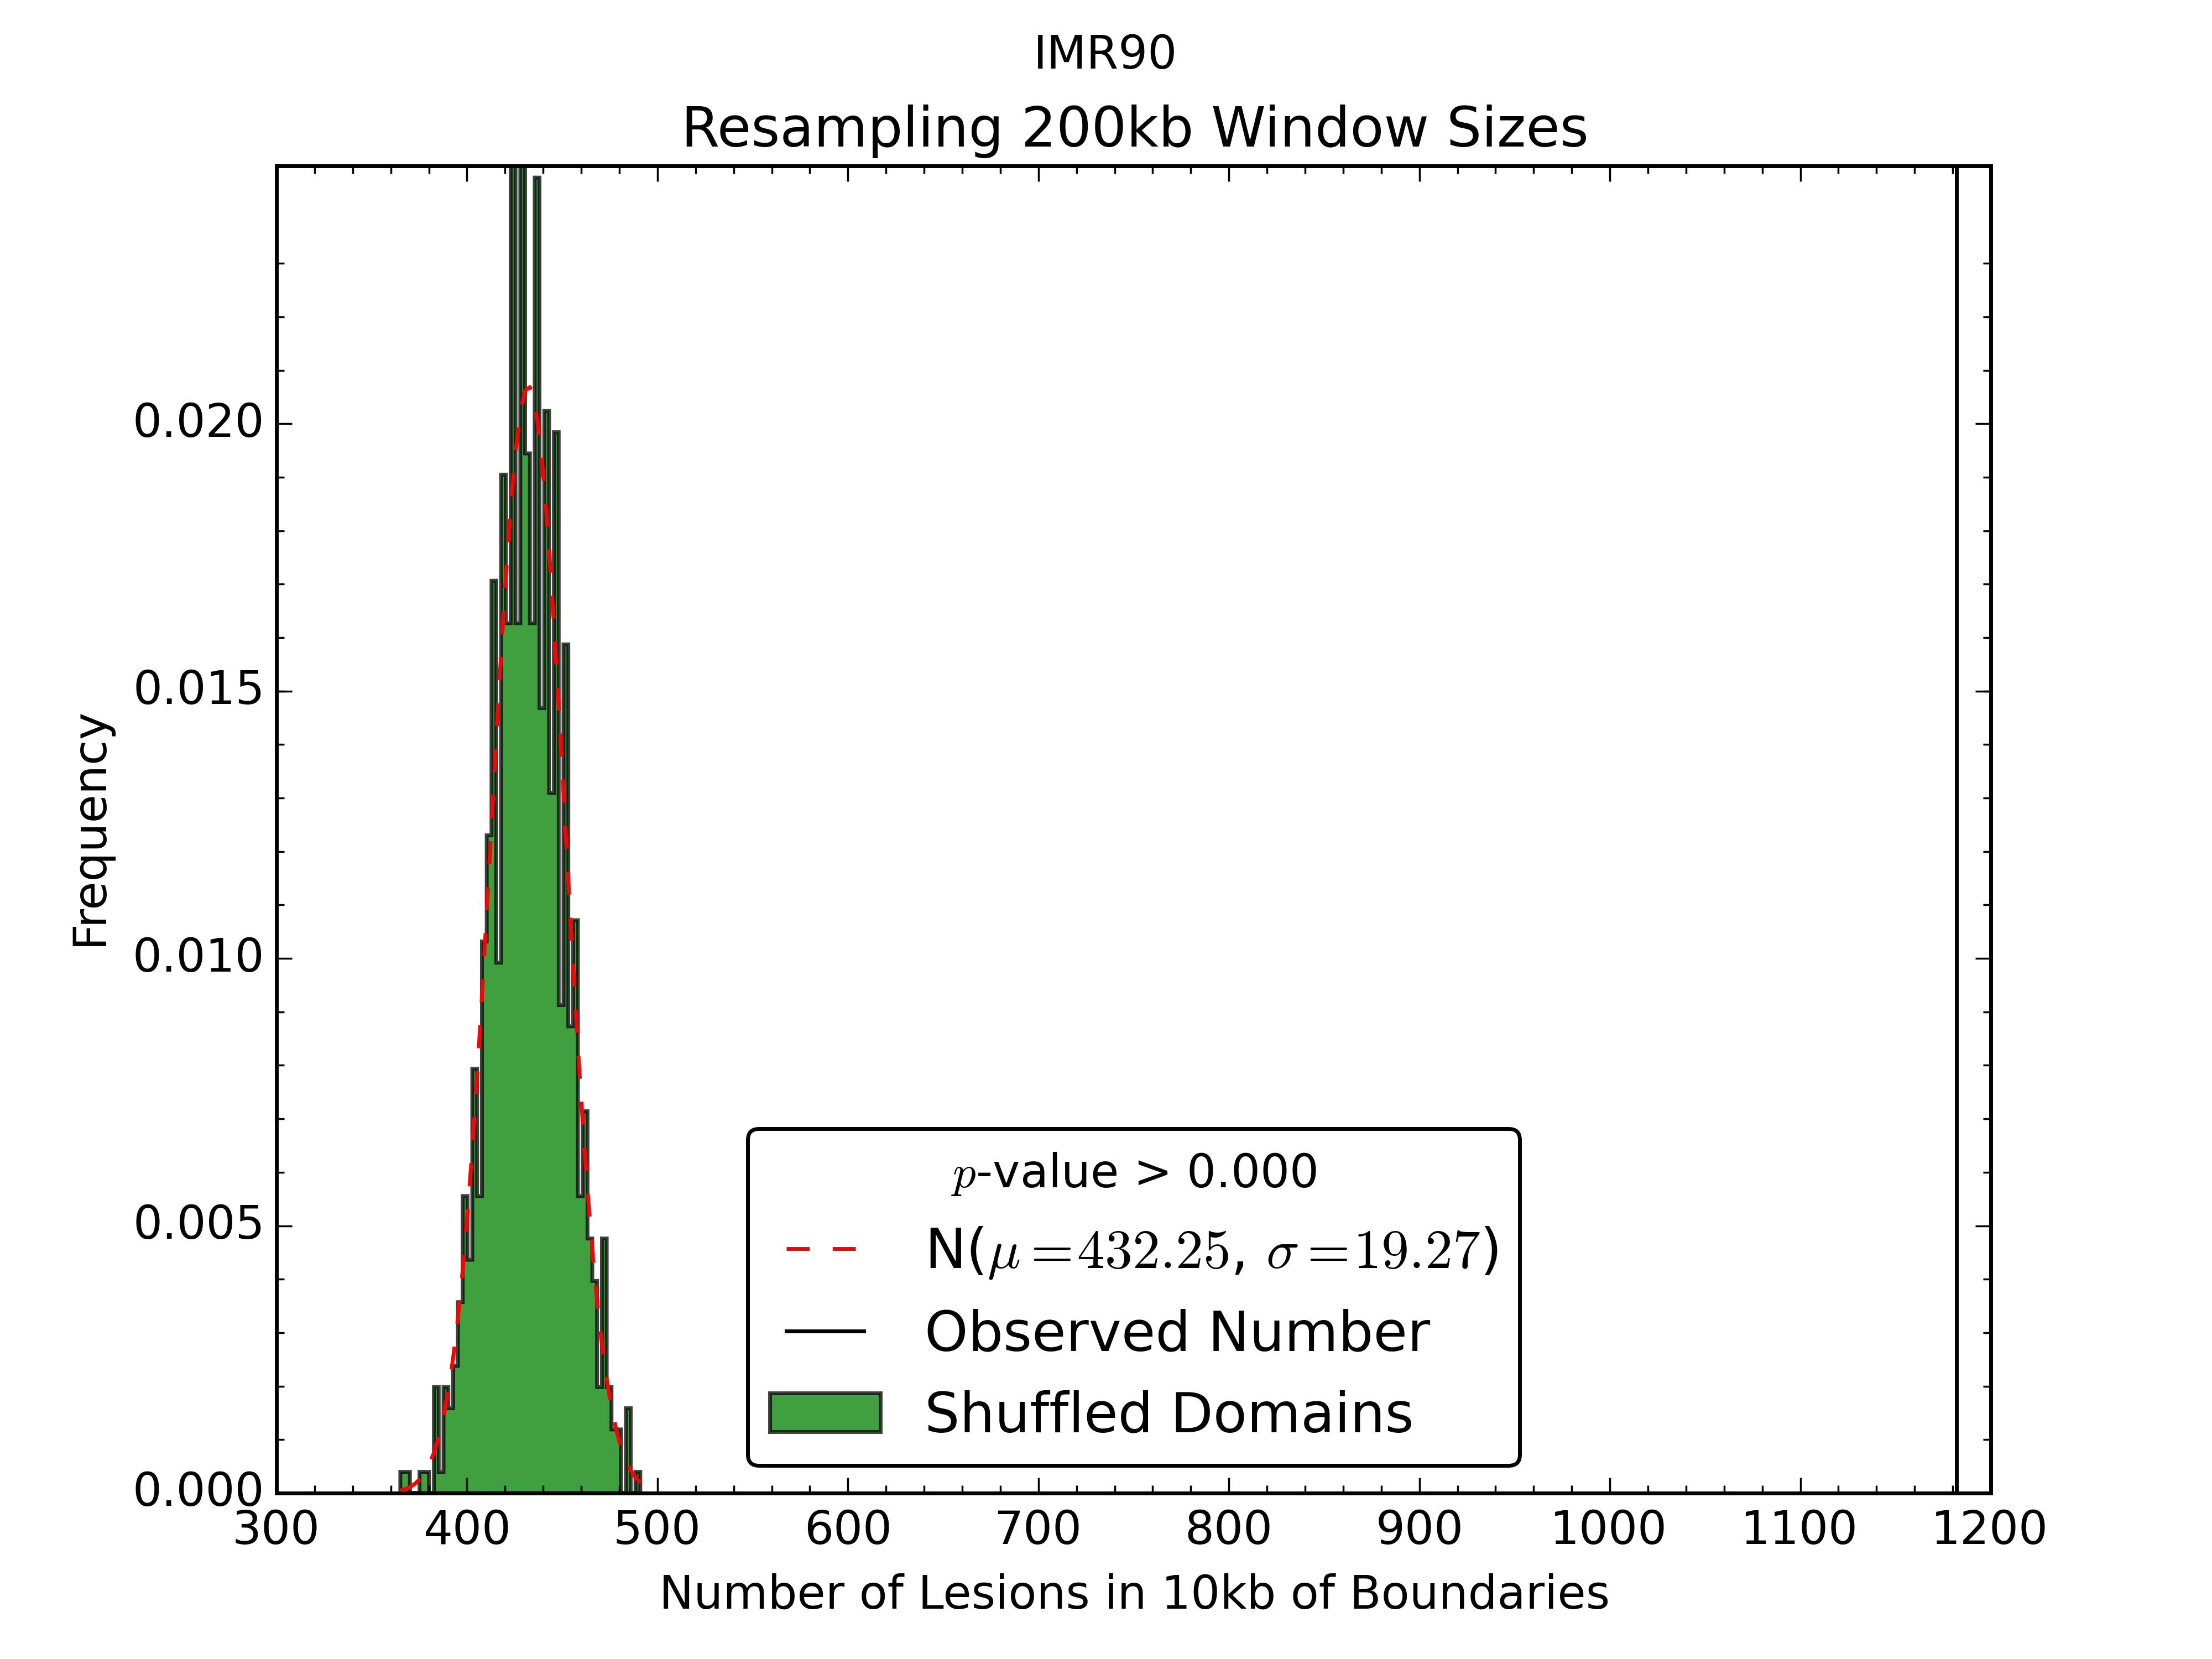
\includegraphics[width=\textwidth]{./figures/supplementary/domains/IMR90boundaries200kbwindows10000kbslop.png}
  \end{minipage}%
  \hfill
  \begin{minipage}{0.5\textwidth}
    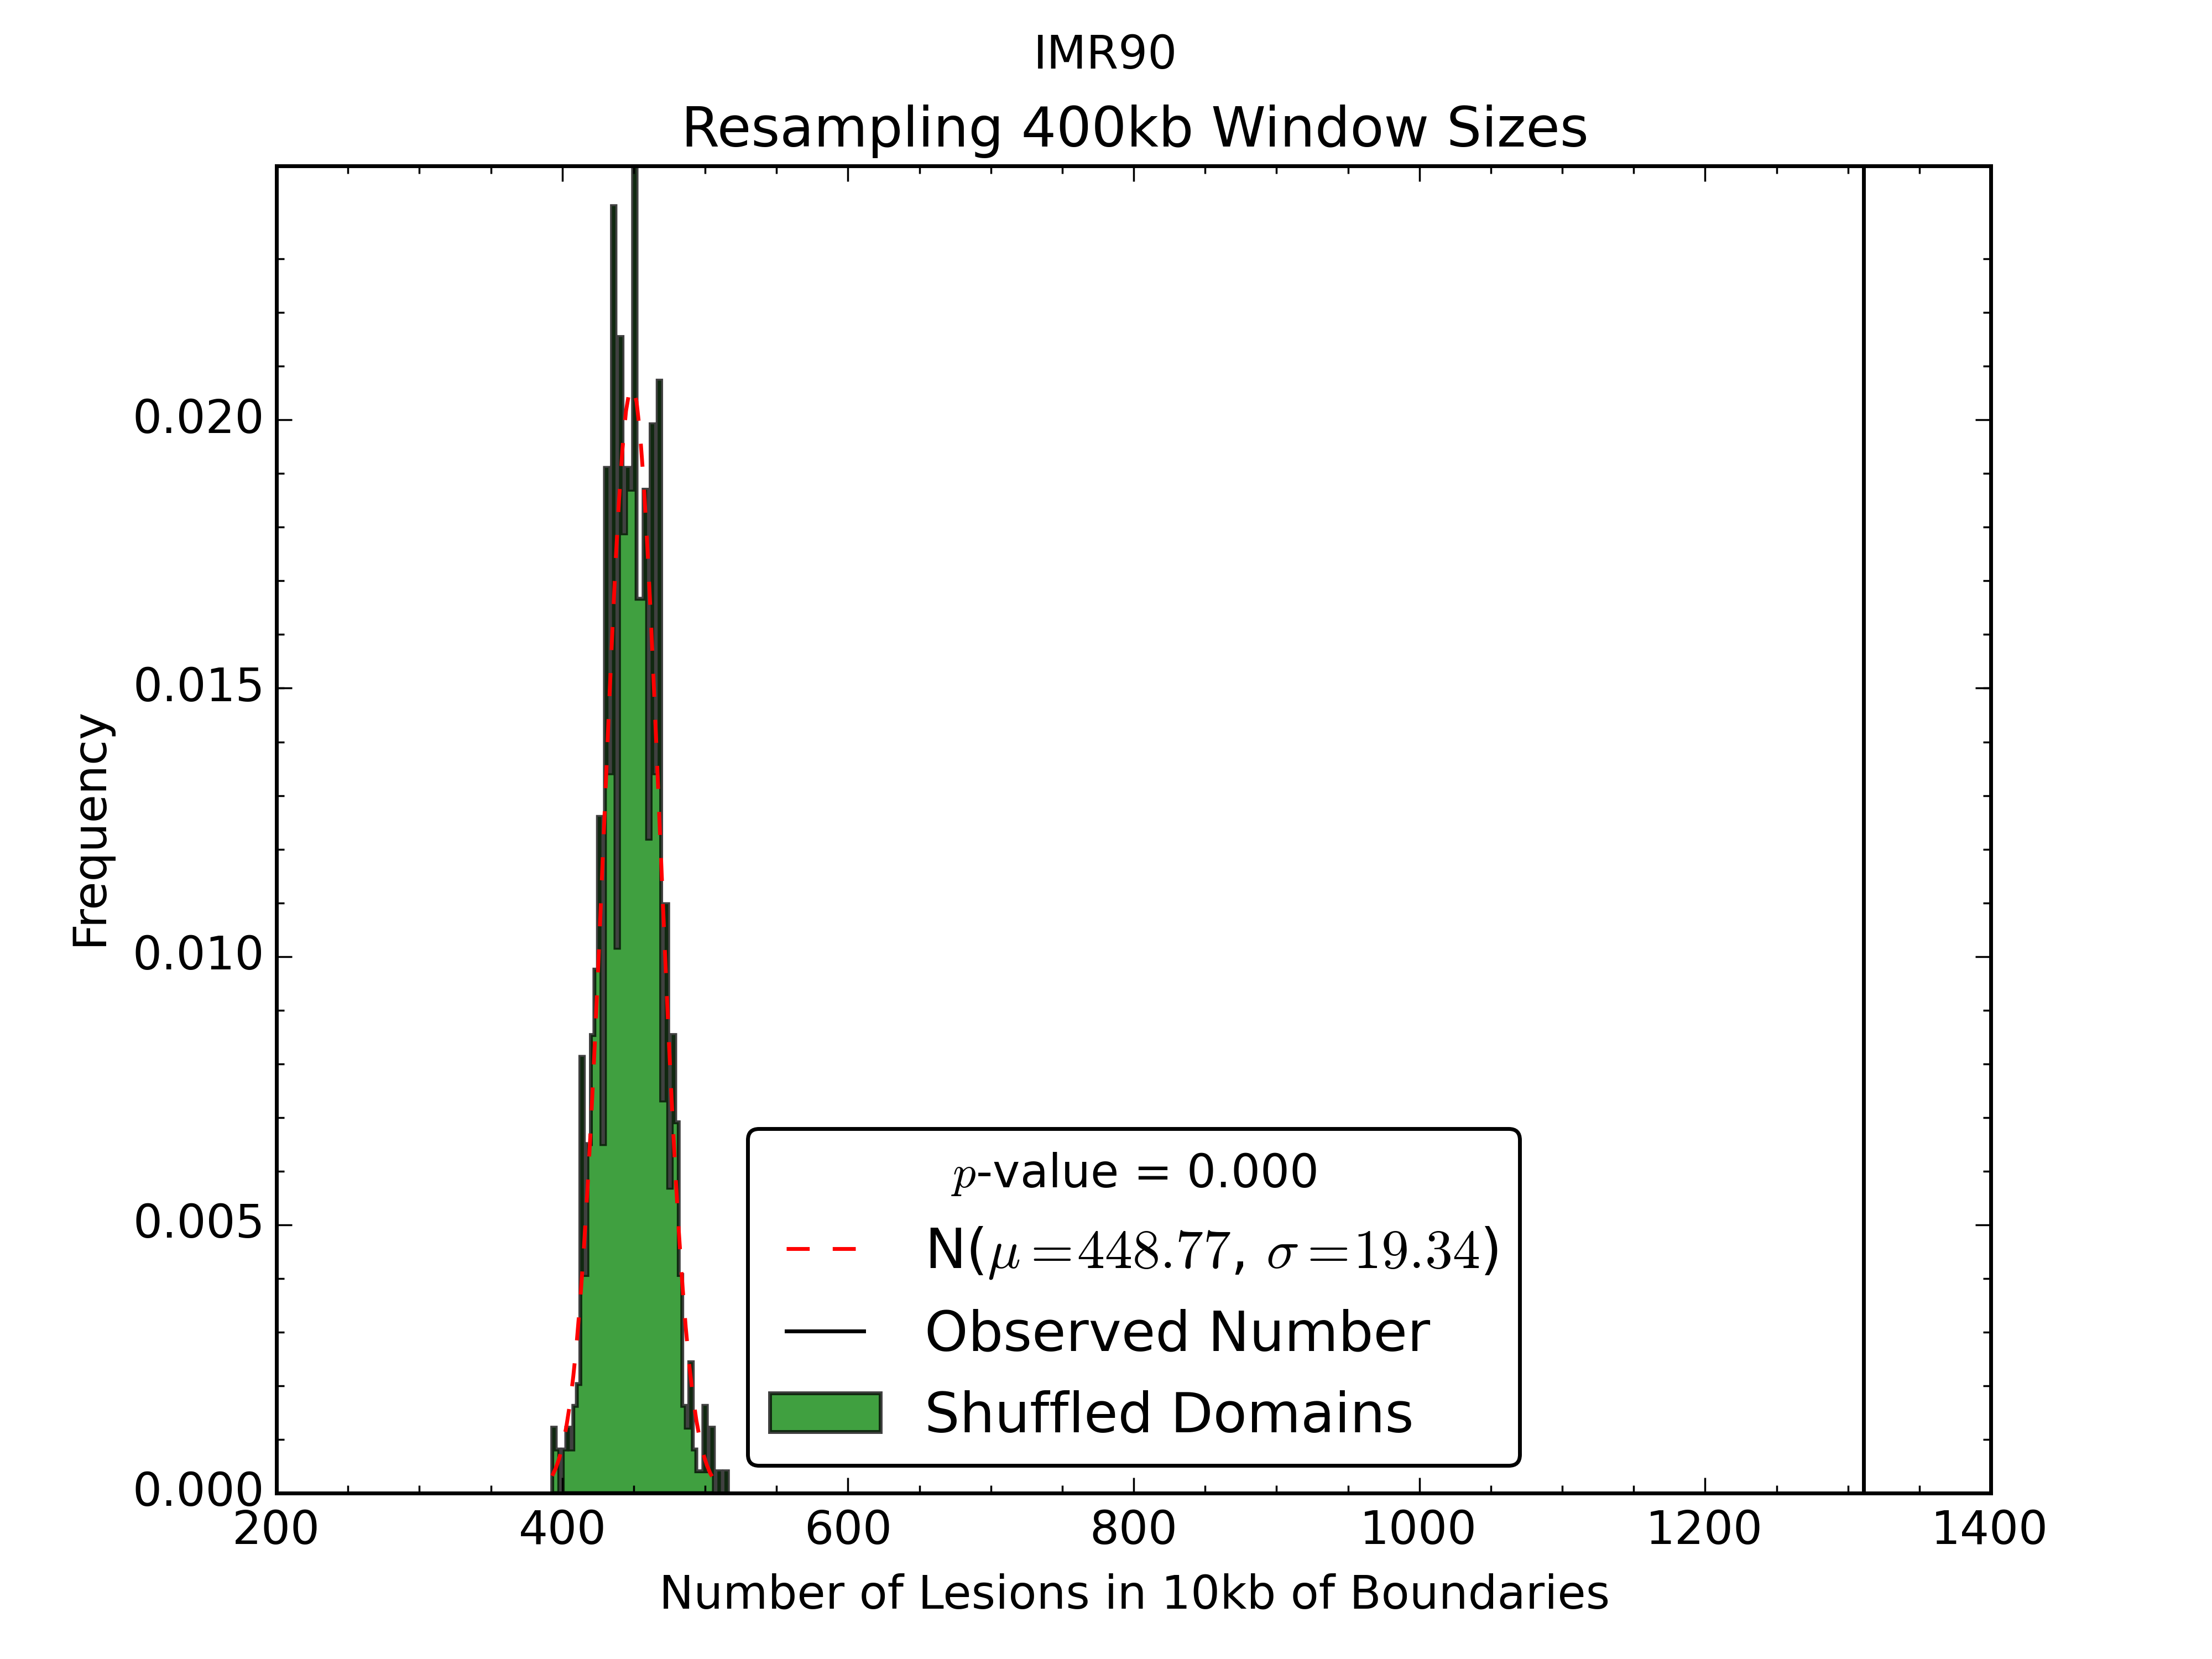
\includegraphics[width=\textwidth]{./figures/supplementary/domains/IMR90boundaries400kbwindows10000kbslop.png}
  \end{minipage}
  \medskip
  \small
  Lesions are clustered around domain boundaries at higher frequencies than expected by chance.  Using shuffling and
  resampling procedures (See Section~\ref{sec:resampling}), we constructed the null hypothesis `lesions are distributed evenly
  throughout boundaries and non-boundary regions.'  In regions of 5kb (top) and 10kb (bottom) around the boundary regions, we are
  able to reject the null hypothesis with negligible $p-$value.
\end{figure}

\begin{figure}[H]
  \caption{Mutation Types from TCGA}
  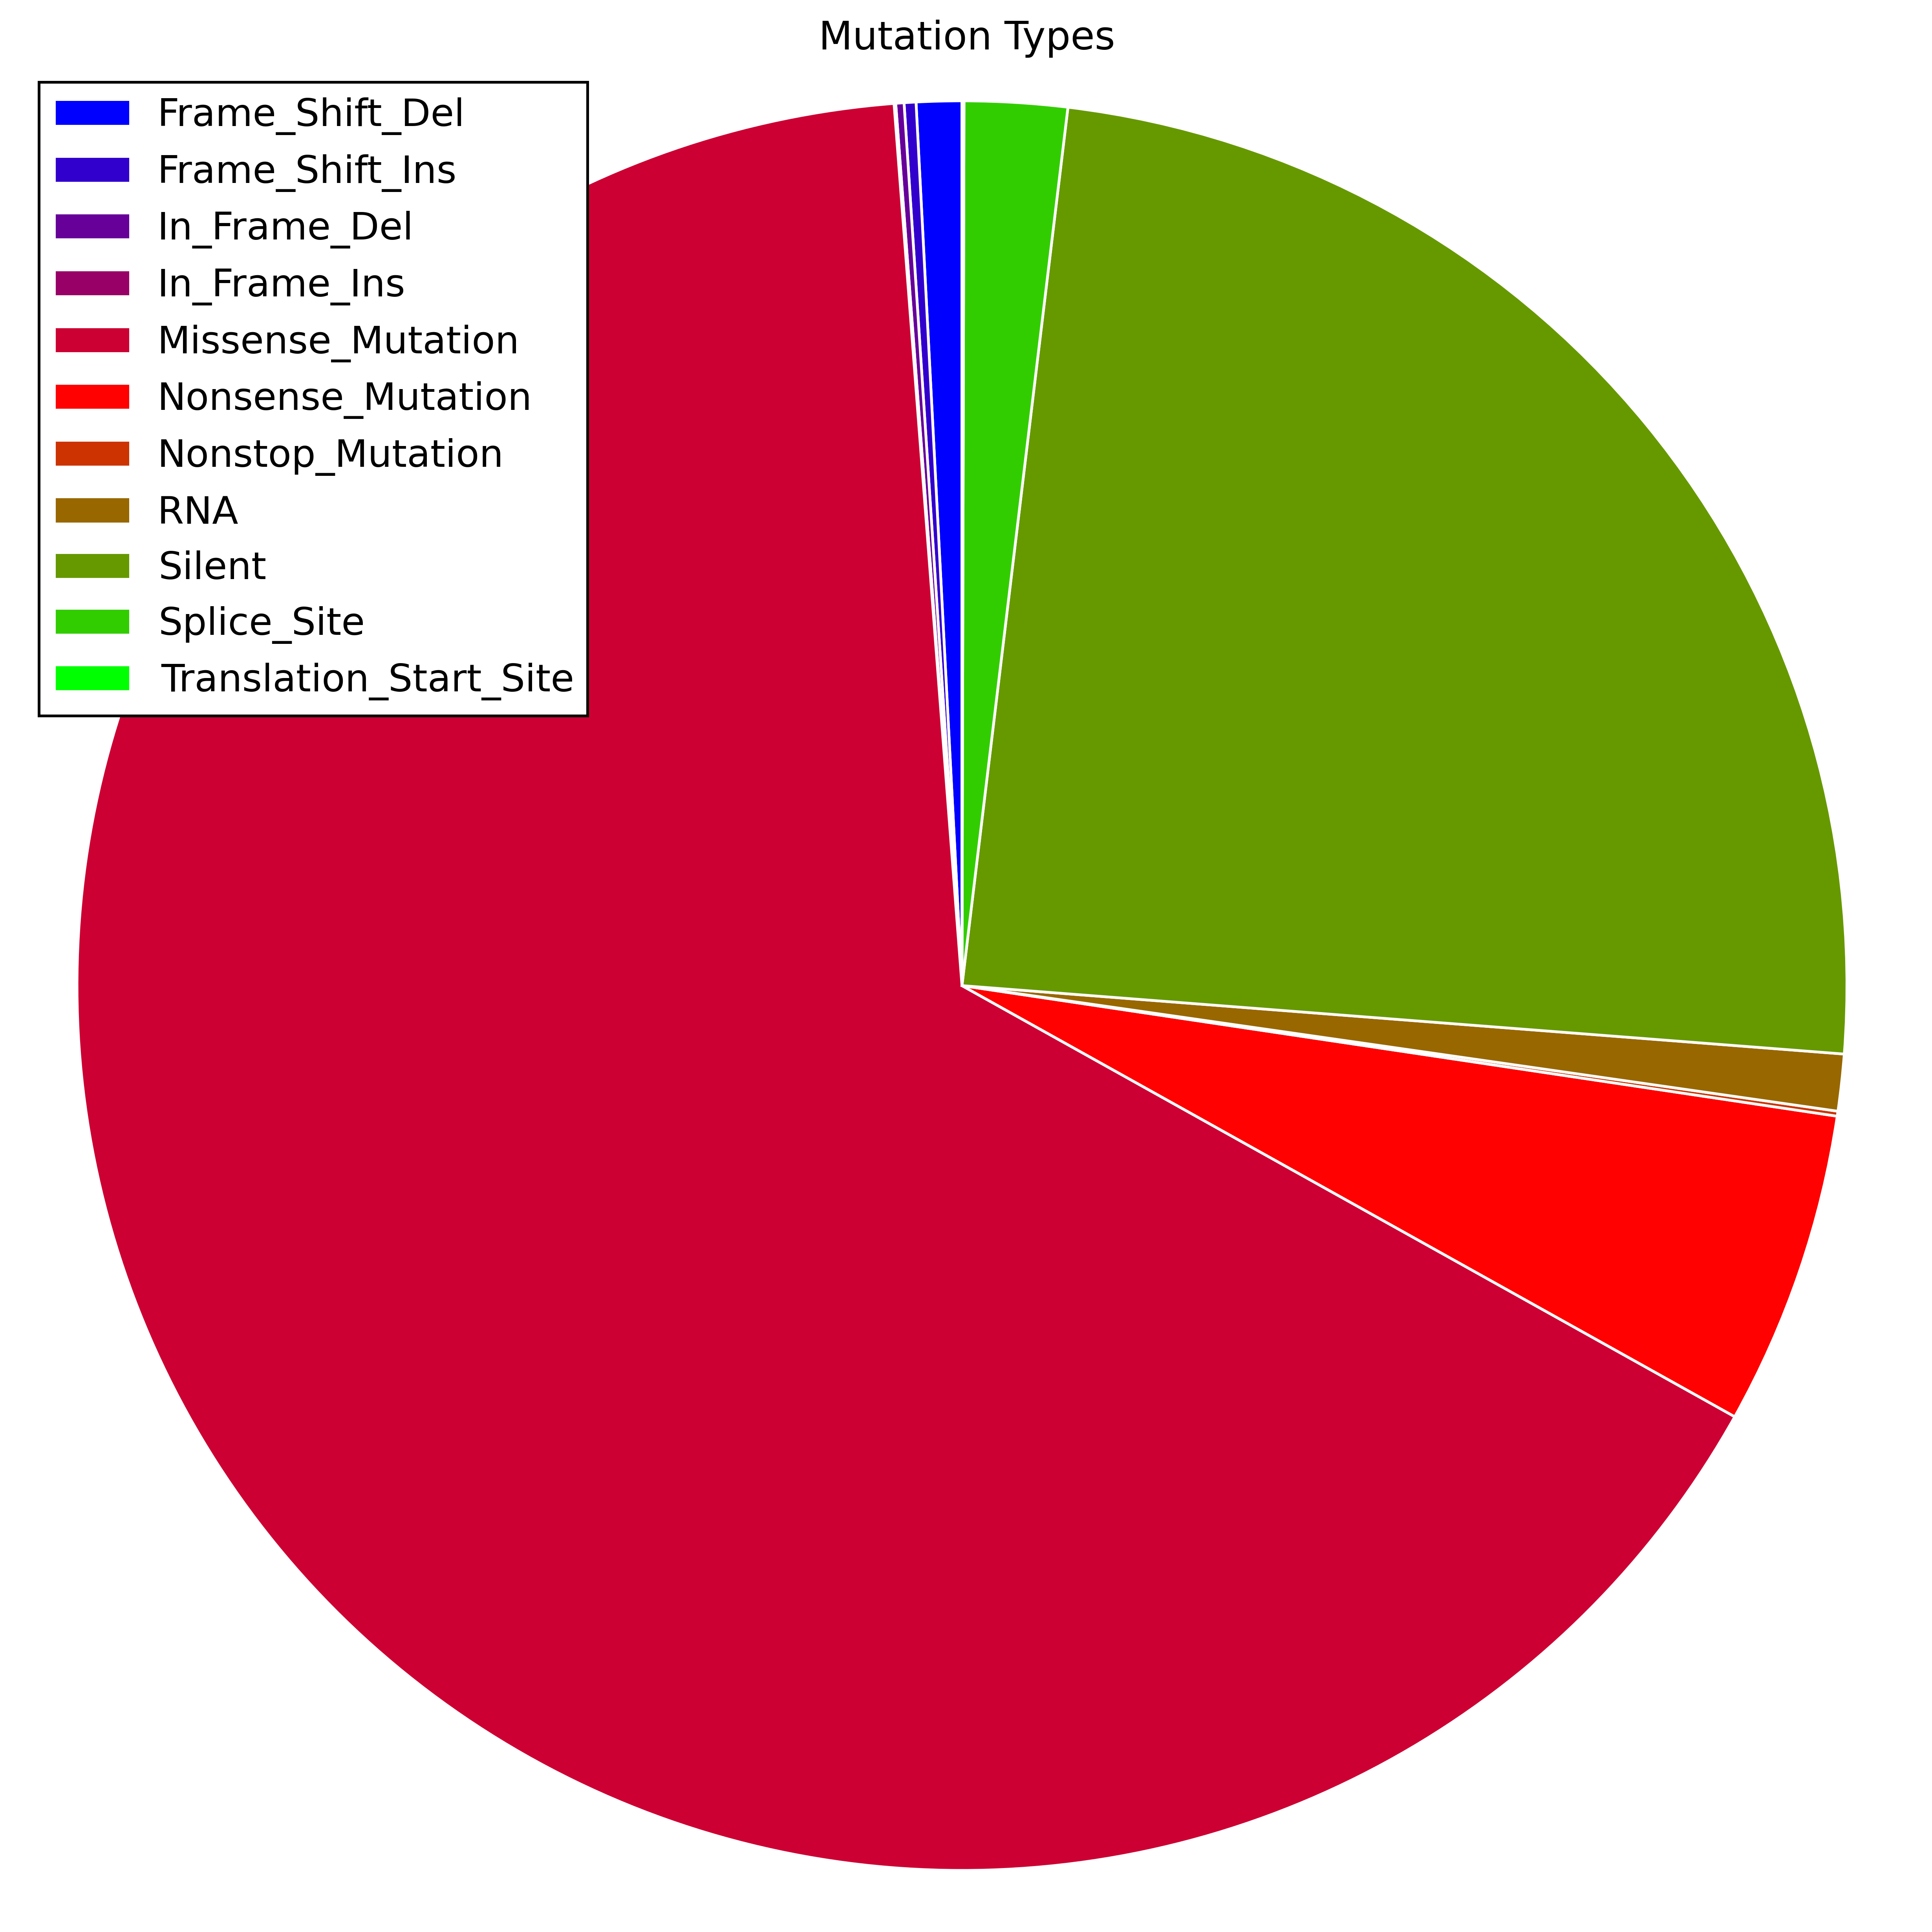
\includegraphics[width=\textwidth]{./figures/supplementary/domains/mutationTypePieChart.png}
\end{figure}

